%%%%%%%%%%%%%%%%%%%%%%%%%%%%%%%%%%%%%%%%%%%%%%%
%
% Template per Elaborato di Laurea
% DISI - Dipartimento di Ingegneria e Scienza dell’Informazione
%
% update 2015-09-10
%
% Per la generazione corretta del 
% pdflatex nome_file.tex
% bibtex nome_file.aux
% pdflatex nome_file.tex
% pdflatex nome_file.tex
%
%%%%%%%%%%%%%%%%%%%%%%%%%%%%%%%%%%%%%%%%%%%%%%%

% formato FRONTE RETRO
\documentclass[epsfig,a4paper,11pt,titlepage,twoside,openany]{book}
\usepackage{epsfig}
\usepackage{plain}
\usepackage{setspace}
\usepackage[paperheight=29.7cm,paperwidth=21cm,outer=1.5cm,inner=2.5cm,top=2cm,bottom=2cm]{geometry} % per definizione layout
\usepackage{titlesec} % per formato custom dei titoli dei capitoli

%%%%%%%%%%%%%%
% supporto lettere accentate
%
%\usepackage[latin1]{inputenc} % per Windows;
\usepackage[utf8x]{inputenc} % per Linux (richiede il pacchetto unicode);
%\usepackage[applemac]{inputenc} % per Mac.

\singlespacing

\usepackage[italian]{babel}

\begin{document}

  % nessuna numerazione
  \pagenumbering{gobble} 
  \pagestyle{plain}

\thispagestyle{empty}

\begin{center}
  \begin{figure}[h!]
    \centerline{
\psfig{file=marchio_unitrento_colore_it_202002.eps,width=0.6\textwidth}}
  \end{figure}

  \vspace{2 cm} 

  \LARGE{Dipartimento di Ingegneria e Scienza dell’Informazione\\}

  \vspace{1 cm} 
  \Large{Corso di Laurea in\\
    Ingegneria Informatica, delle Comunicazioni ed Elettronica
    %Informatica
    %Ingegneria dell'Informazione e delle Comunicazioni
    %Ingegneria dell'Informazione e Organizzazione d'Impresa
    %Ingegneria Elettronica e delle Telecomunicazioni
  }

  \vspace{2 cm} 
  \Large\textsc{Elaborato finale\\} 
  \vspace{1 cm} 
  \Huge\textsc{Static and reconfigurable metasurfaces\\}


  \vspace{2 cm} 
  \begin{tabular*}{\textwidth}{ c @{\extracolsep{\fill}} c }
  \Large{Supervisore} & \Large{Laureando}\\
  \Large{......}& \Large{Tairovski Denis}\\
  \end{tabular*}

  \vspace{2 cm} 

  \Large{Anno accademico 21/22}
  
\end{center}



  \clearpage
 
%%%%%%%%%%%%%%%%%%%%%%%%%%%%%%%%%%%%%%%%%%%%%%%%%%%%%%%%%%%%%%%%%%%%%%%%%%
%%%%%%%%%%%%%%%%%%%%%%%%%%%%%%%%%%%%%%%%%%%%%%%%%%%%%%%%%%%%%%%%%%%%%%%%%%
%% Nota
%%%%%%%%%%%%%%%%%%%%%%%%%%%%%%%%%%%%%%%%%%%%%%%%%%%%%%%%%%%%%%%%%%%%%%%%%%
%% Sezione Ringraziamenti opzionale
%%%%%%%%%%%%%%%%%%%%%%%%%%%%%%%%%%%%%%%%%%%%%%%%%%%%%%%%%%%%%%%%%%%%%%%%%%
%%%%%%%%%%%%%%%%%%%%%%%%%%%%%%%%%%%%%%%%%%%%%%%%%%%%%%%%%%%%%%%%%%%%%%%%%%
  \thispagestyle{empty}

\begin{center}
  {\bf \Huge Acknowledgments}
\end{center}

\vspace{4cm}

  I want to express my gratitude to all the people that supported me during these years of hard work. 
  A special thanks to Salucci Marco and Benoni Arianna, who followed my work with particular care from the very beginning.\\
 I would like to offer my special thanks to my family, who supported me in every way possible, especially during my hard times.\\
  And last but not least, I am deeply grateful to my best friends, who encouraged me to believe in myself.
  \bigskip
  

\begin{FlushRight}
\emph{It's not about the journey. It's about the people you meet.\\
"Del Close"}
\end{FlushRight}
  \clearpage
  \pagestyle{plain} % nessuna intestazione e pie pagina con numero al centro

  
  % inizio numerazione pagine in numeri arabi
  \mainmatter

%%%%%%%%%%%%%%%%%%%%%%%%%%%%%%%%%%%%%%%%%%%%%%%%%%%%%%%%%%%%%%%%%%%%%%%%%%
%%%%%%%%%%%%%%%%%%%%%%%%%%%%%%%%%%%%%%%%%%%%%%%%%%%%%%%%%%%%%%%%%%%%%%%%%%
%% Nota
%%%%%%%%%%%%%%%%%%%%%%%%%%%%%%%%%%%%%%%%%%%%%%%%%%%%%%%%%%%%%%%%%%%%%%%%%%
%% Si ricorda che il numero massimo di facciate e' 30.
%% Nel conteggio delle facciate sono incluse 
%%   indice
%%   sommario
%%   capitoli
%% Dal conteggio delle facciate sono escluse
%%   frontespizio
%%   ringraziamenti
%%   allegati    
%%%%%%%%%%%%%%%%%%%%%%%%%%%%%%%%%%%%%%%%%%%%%%%%%%%%%%%%%%%%%%%%%%%%%%%%%%
%%%%%%%%%%%%%%%%%%%%%%%%%%%%%%%%%%%%%%%%%%%%%%%%%%%%%%%%%%%%%%%%%%%%%%%%%%

    % indice
    \tableofcontents
    \clearpage
    
    
          
    % gruppo per definizone di successione capitoli senza interruzione di pagina
    \begingroup
      % nessuna interruzione di pagina tra capitoli
      % ridefinizione dei comandi di clear page
      \renewcommand{\cleardoublepage}{} 
      \renewcommand{\clearpage}{} 
      % redefinizione del formato del titolo del capitolo
      % da formato
      %   Capitolo X
      %   Titolo capitolo
      % a formato
      %   X   Titolo capitolo
      
      \titleformat{\chapter}
        {\normalfont\Huge\bfseries}{\thechapter}{1em}{}
        
      \titlespacing*{\chapter}{0pt}{0.59in}{0.02in}
      \titlespacing*{\section}{0pt}{0.20in}{0.02in}
      \titlespacing*{\subsection}{0pt}{0.10in}{0.02in}
      
      % sommario
      \newpage
\chapter*{Summary} % senza numerazione
\label{Summary}

\addcontentsline{toc}{chapter}{Summary} % da aggiungere comunque all'indice

This discourse aims to describe and analyze the work behind Meta-Surfaces. A mathematical description of various meta-surfaces is provided, emphasizing the need to create a Meta-Surface adapted to the environment where is going to be placed. After that, a practical description is provided, having an existing scenario to be improved. To achieve that, various Meta-Surfaces are going to be employed, having different scenarios discussed. To obtain the descripted goal, various tools are used, such as the Feko Winprop Suite, the Ansys HFSS Suite and GNUPlot scripts provided. As for the conclusions, the goal has been greatly achieved, with an extended discussion for every step.

%%%%%%%%%%%%%%%%%%%%%%%%%%%%%%%%%%%%%%%%%%%%%%%%%%%%%%%%%%%%%%%%%%%%%%%%%%
%%%%%%%%%%%%%%%%%%%%%%%%%%%%%%%%%%%%%%%%%%%%%%%%%%%%%%%%%%%%%%%%%%%%%%%%%%
%% Nota
%%%%%%%%%%%%%%%%%%%%%%%%%%%%%%%%%%%%%%%%%%%%%%%%%%%%%%%%%%%%%%%%%%%%%%%%%%
%% Sommario e' un breve riassunto del lavoro svolto dove si descrive 
%% l’obiettivo, l’oggetto della tesi, le metodologie e 
%% le tecniche usate, i dati elaborati e la spiegazione delle conclusioni 
%% alle quali siete arrivati.
%% Il sommario dell’elaborato consiste al massimo di 3 pagine e deve contenere le seguenti informazioni: 
%%   contesto e motivazioni
%%   breve riassunto del problema affrontato
%%   tecniche utilizzate e/o sviluppate
%%   risultati raggiunti, sottolineando il contributo personale del laureando/a
%%%%%%%%%%%%%%%%%%%%%%%%%%%%%%%%%%%%%%%%%%%%%%%%%%%%%%%%%%%%%%%%%%%%%%%%%%
%%%%%%%%%%%%%%%%%%%%%%%%%%%%%%%%%%%%%%%%%%%%%%%%%%%%%%%%%%%%%%%%%%%%%%%%%%      
      
      %%%%%%%%%%%%%%%%%%%%%%%%%%%%%%%%
      % lista dei capitoli
      %
      % \input oppure \include
      %
      \chapter{In ante nulla, vestibulum a}
\label{cha:intro}

Lorem ipsum dolor sit amet, consectetur adipiscing elit. Donec sed nunc orci. Aliquam nec nisl vitae sapien pulvinar dictum quis non urna. Suspendisse at dui a erat aliquam vestibulum. Quisque ultrices pellentesque pellentesque. Pellentesque egestas quam sed blandit tempus. Sed congue nec risus posuere euismod. Maecenas ut lacus id mauris sagittis egestas a eu dui. Class aptent taciti sociosqu ad litora torquent per conubia nostra, per inceptos himenaeos. Pellentesque at ultrices tellus. Ut eu purus eget sem iaculis ultricies sed non lorem. Curabitur gravida dui eget ex vestibulum venenatis. Phasellus gravida tellus velit, non eleifend justo lobortis eget. 
\cite{coulouris}

Donec eu ipsum id lorem consectetur luctus ac a nisi. Curabitur volutpat, metus id porta ultrices, felis lacus consectetur justo, ut gravida arcu ex in purus. Pellentesque vitae sapien ac nisl porttitor pellentesque eu sed elit. Sed maximus lectus eu eros ultricies accumsan. Quisque congue, nisi in dictum cursus, ante nisl molestie eros, in ultrices eros tellus sit amet augue. Interdum et malesuada fames ac ante ipsum primis in faucibus. Nam finibus leo sit amet purus vehicula, eget facilisis turpis convallis. Vivamus varius tincidunt turpis, id venenatis arcu maximus ut. Aenean euismod eros ac nibh facilisis, nec imperdiet ex suscipit.
\cite{dalal}


\section{Pellentesque habitant morbi tristique senectus}
\label{sec:context}

Lorem ipsum dolor sit amet, consectetur adipiscing elit. Donec sed nunc orci. Aliquam nec nisl vitae sapien pulvinar dictum quis non urna. Suspendisse at dui a erat aliquam vestibulum. Quisque ultrices pellentesque pellentesque. Pellentesque egestas quam sed blandit tempus. Sed congue nec risus posuere euismod. Maecenas ut lacus id mauris sagittis egestas a eu dui. Class aptent taciti sociosqu ad litora torquent per conubia nostra, per inceptos himenaeos. Pellentesque at ultrices tellus. Ut eu purus eget sem iaculis ultricies sed non lorem. Curabitur gravida dui eget ex vestibulum venenatis. Phasellus gravida tellus velit, non eleifend justo lobortis eget.
\cite{ictbusiness}
\cite{donoho}

\section{Nullam et justo vitae nisi}
\label{sec:problem}

Lorem ipsum dolor sit amet, consectetur adipiscing elit. Donec sed nunc orci. Aliquam nec nisl vitae sapien pulvinar dictum quis non urna. Suspendisse at dui a erat aliquam vestibulum. Quisque ultrices pellentesque pellentesque. Pellentesque egestas quam sed blandit tempus. Sed congue nec risus posuere euismod. Maecenas ut lacus id mauris sagittis egestas a eu dui. Class aptent taciti sociosqu ad litora torquent per conubia nostra, per inceptos himenaeos. Pellentesque at ultrices tellus. Ut eu purus eget sem iaculis ultricies sed non lorem. Curabitur gravida dui eget ex vestibulum venenatis. Phasellus gravida tellus velit, non eleifend justo lobortis eget.



      \textcolor{white}{\section*{}}
\chapter{State-of-Art Analysis}
\label{cha:State-of-art}
This Section is focused on the detailed analysis (HL-SoA) of the design methodology proposed in \cite{Oliveri:2021}.
\begin{table}[H]
\centering\footnotesize
\resizebox{\textwidth}{!}{\begin{tabular}{|p{0.1\linewidth}|p{0.07\linewidth}|p{0.45\textwidth}|p{0.15\linewidth}|p{0.15\linewidth}|} 
 \hline
 \textbf{ID} & \textbf{Year} & \textbf{Title} & \textbf{Journal} & \textbf{Authors}\\ 
 \hline
 Oliveri.2021 & 2021 & Holographic Smart EM Skins for Advanced Beam Power Shaping in Next Generation Wireless Environments & IEEE J. Multiscale Multiphys. Comput. Tech & G. Oliveri, P. Rocca, M. Salucci and A. Massa\\
 \hline
\end{tabular}} 
\end{table}
\section{Holographic Smart EM Skins for Advanced Beam Power Shaping in Next Generation Wireless Environments \cite{Oliveri:2021}}
\subsection{Motivation and Principles}
As the technology moves forward, a much larger quantity of data needs to travel. Nowadays, everything can be done using a mobile device and in order to secure a stable connection, the wireless cellular system need to fulfill a various number of requirements, such as transfer speed, flexibility, coverage, reliability and quality of service. Since the urban environments is in a continuous state of change, the Base Station is incapable to rely on itself. Since the upgrading of the upgrading of the technology behind the Base Stations or the cellular device has its limits, it's fundamental to use the urban environment as efficiently as possible. Every urban environment as much wider and taller building that interrupts the Line-Of-Sight between Base Station and User. That's the main point of creating a Smart Electromagnetic Environment (SEE). Thanks to a SEE, the environment acquires the ability to adapt itself to help fulfilling all those previous citated requirements and, subsequently, the scenario becomes a controllable part of a wireless system . In order to adapt the environment, we use thin meta-surfaces operating as Smart Electromagnetic (EM) Skins. Thanks to this technology, the manipulation of the reflected/transmitted wavefront, at a meta-atomic level, to overcome Snell's Law, is possible. Snell's Law states that, in very simple terms, “input and output angle are the same”. This constraint implies a large set of unconventional phenomena, such as anomalous reflections or perfect absorption. On the other hand, dynamically adjustable artificial materials operating as Reconfigurable Intelligent Surfaces (RIS) give the control of the reflected wave properties in realtime, implying non-negligible implementation complexity, costs and power consumption. On the contrary, static passive smart EM skins (SPSSs) imply no running costs after installation and they potentially have advanced beamforming and contoured footprint radiation capabilities when featuring a holographic layout, therefore enabling to increase the coverage and reduce blind spot regions in urban wireless communications. The negative side of SPSSs are its degrees-of-freedom (DoFs); since the DoFs are severely constrained in terms of the final layout complexity, its design is very challenging. One characteristic that SPSSs need to have is its size: the size of a SPSSs need to be large enough to reflect an adequate quantity of power to the coverage area but it needs to respect some size limitations in order to not be excessively big. Furthermore, another DoFs that could be considered is the surface orientation; even though its control it’s limited, its usability to enhance the performance of the SPSSs,  respecting the incident direction of the illuminating beam, is necessary. The objective of this paper is to give some indications on the feasibility of simple and inexpensive holographic SPSSs suitable for advanced wave manipulation and beamforming. To achieve this, the need to formulate a complex multiscale EM design problem within the Generalized Sheet Transition Condition (GSTC) theoretical framework is needed. A phase-only inverse source (IS) is adopted to generalize concepts, such as the non-uniqueness of the radiation operator due to the existence of non-radiating (NR) currents for reflect-array engineering to the synthesis of a holographic meta-surface working in the SEE scenario. The footprint coverage capabilities of the smart EM skin arre successively optimized by combining:
\begin{itemize}
\item a local search approach, based on Iterative Projection Technique (IPT): aims at deducing the reference/ideal surface currents affording the user-defined footprint pattern;
\item a customized version of the System-by-Design (SbD) paradigm: sets the descriptors of the SPSSs for matching these reference currents
\end{itemize}
Such methodological choices in the implementation of a synthesis method for SPSSs are driven by:
\begin{itemize}
\item accuracy of GSTC theory in accounting of the comples EM response of smart skins in the SEE environment;
\item effectiveness of the SbD in handling complex multi-scale desing problems;
\item intrinsic advantages of exploiting an IS formulation when determining surface currents;
\end{itemize}
Consequently, the main innovative contributions of this work lie in:
\begin{itemize}
\item customization of the SbD paradigm within the GSTC framework;
\item combination of the SbD-based technique and of an IPT-based source synthesis process to afford complex pattern footprints with simple and inexpensive SPSS layouts;
\item numerical assessment of the effectiveness of the proposed approach as well as of the feasibility of holographic SPSSs able to generate complex footprints.
\end{itemize}
To asses correctly the stated problem, the following auxiliary papers
\begin{table}[H]
\centering
\resizebox{\textwidth}{!}{\begin{tabular}{|p{0.15\linewidth}|p{0.07\linewidth}|p{0.55\textwidth}|p{0.15\linewidth}|p{0.1\linewidth}|} 
 \hline
 \textbf{ID} & \textbf{Year} & \textbf{Title} & \textbf{Journal} & \textbf{Authors}\\ 
 \hline
 Yang.2021 & 2021 & Surface Electromagnetics With Applications in Antenna, Microwave and Optical Engineering & Cambridge Univ. Press & F. Yang and Y. Rahmat-Sanni \\
 \hline
 Salucci.2018 & 2018 & Synthesis of shaped beam reflectarrays with constrained geometry by exploiting non-radiating surface currents & IEEE Trans. Antennas Propag & M. Salucci et al.\\
 \hline
\end{tabular}} 
\end{table}
will be used, since they contain a needed case study. It's worth pointing out that the \cite{Oliveri:2021} has more references, but for the sake of the formulation, only these are needed, since they contain important experiments that cannot be vastly explained in this discussion.
\subsection{Mathematical Formulation and Design Formulas}
\label{sub:Mathematical-And-Design-Formulas}
\begin{figure}[H]
\centering
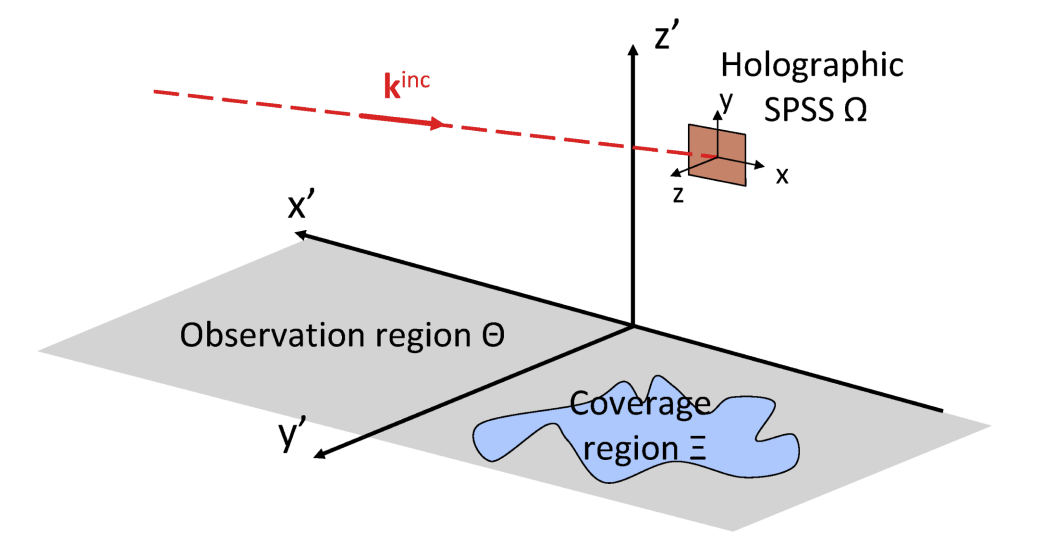
\includegraphics[scale=0.35]{./Figure/Figure01.png}
\label{cap:Geom}
\caption{\footnotesize Problem geometry. Sketch of the Smart EM skin scenario illustrating the incident wave vector $k^{inc}$, the observation region $\Theta$, the coverage region $\Xi$ and the holographic SPSSs area with both local $(x, y, z)$ and global $(x^{'}, y^{'}, z^{'})$ coordinates.}
\end{figure}
With reference to the scenario in \ref{cap:Geom} and without loss
of generality, let us consider a \emph{SPSSs} componsed by $P\times Q$
meta-film unit cells located at the positions $\{\mathbf{\mathbf{r}}_{pq}\in\Omega;p=1,\cdots,P;q=1,\cdots,Q\}$,$\Omega$
being the smart sking aperture/support and illuminated by an incident
plane wave impinging from the angular direction $(\theta^{inc},\varphi^{inc})$
whose associated electric magnetic are

\begin{equation}
\mathbf{E}^{inc}(\mathbf{r})\triangleq(E_{\perp}^{inc}\mathbf{\hat{e}}_{\perp}+E_{\parallel}^{inc}\mathbf{\hat{e}}_{\parallel})\exp(-j\mathbf{k}^{inc}\cdot\mathbf{r})\label{eq:1}\end{equation}


and

\begin{equation}
\mathbf{H}^{inc}(\mathbf{r})\triangleq\frac{1}{\eta_{0}k_{0}}\mathbf{k}^{inc}\times\mathbf{E}^{inc}(\mathbf{r})\label{eq:2}\end{equation}


respectively, $\mathbf{k}^{inc}$ being the incident wave vector 

\begin{equation}
\mathbf{k}^{inc}\triangleq-k_{0}[\sin(\theta^{inc})\cos(\varphi^{inc})\mathbf{\hat{x}}+\sin(\theta^{inc})\sin(\varphi^{inc})\mathbf{\hat{y}}+\cos(\theta^{inc})\mathbf{\hat{z}}]\label{eq:3}\end{equation}


while: $\mathbf{r}=(x,y,z)$ is the metasurface local coordinate; $k_{0}$ is the free-space wavenumber; $\eta_{0}$ is the intrinsic impedance; $\mathbf{\hat{e}}_{\perp}=\frac{\mathbf{k}^{inc}\times\mathbf{\hat{n}}}{|\mathbf{k}^{inc}\times\mathbf{\hat{n}}|}$ is the perpendicular unit vector; $\mathbf{\hat{e}}_{\parallel}=\frac{\mathbf{\hat{e}}_{\perp}\times\mathbf{k}^{inc}}{|\mathbf{\hat{e}}_{\perp}\times\mathbf{k}^{inc}|}$ is the parallel unit vector; $E_{\perp}^{inc}$ and $E_{\parallel}^{inc}$ are the corresponding complex-valued coefficients; $\mathbf{\hat{n}}$ is the normal to the smart skin surface; $\mathbf{|\cdot|}$is the vector magnitude operator.\\
In the far-field, the electric field reflected by the \emph{SPSSs}
is given by

\begin{equation}
\mathbf{E}^{FF}(\mathbf{r})\approx\mathcal{G}[\mathbf{J}^{e}(\mathbf{r}),\mathbf{J}^{m}(\mathbf{r})]\triangleq\frac{jk_{0}}{4\pi}\frac{\exp(-ik_{0}|\mathbf{r}|)}{|\mathbf{r}|}\times\int_{\Omega}\{\mathbf{\hat{r}}\times[\eta_{0}\mathbf{\hat{r}}\times\mathbf{J}^{e}(\tilde{\mathbf{r}})+\mathbf{J}^{m}(\mathbf{\tilde{r}})]\exp(jk_{0}\mathbf{\hat{r}}\cdot\mathbf{\tilde{r}})\} d\mathbf{\tilde{r}}\label{eq:4}\end{equation}


where $\mathbf{\hat{r}}=\frac{\mathbf{r}}{|\mathbf{r}|}$.

Moreover, the effective equivalent electric/magnetic surface current
, $\mathbf{J}^{e}(\mathbf{r})/\mathbf{J}^{m}(\mathbf{r})$, is computed
according to the \emph{GSTC} as follows:

\begin{equation}
\mathbf{J}^{e}(\mathbf{r})=j\omega\mathbf{B_{t}^{e}}(\mathbf{r})-\mathbf{\hat{n}}\times\nabla_{t}B_{n}^{m}(\mathbf{r})\quad\mathbf{r}\in\Omega\label{eq:5}\end{equation}


\begin{equation}
\mathbf{J}^{e}(\mathbf{r})=j\omega\mu_{0}\mathbf{B_{t}^{m}}(\mathbf{r})+\mathbf{\hat{n}}\times\nabla_{t}\frac{B_{n}^{e}(\mathbf{r})}{\varepsilon_{0}}\quad\mathbf{r}\in\Omega\label{eq:6}\end{equation}


where:

\begin{itemize}
\item $\varepsilon_{0}$ is the free-space permeattivity
\item $\mu_{0}$is the free-space permeability
\item $\mathbf{B}^{e}(\mathbf{r})=\mathbf{B}_{t}^{e}(\mathbf{r})+B_{n}^{e}(\mathbf{r})\mathbf{\hat{n}}$
is the electric polarization surface density
\item $\mathbf{B}^{m}(\mathbf{r})=\mathbf{B}_{t}^{m}(\mathbf{r})+B_{n}^{m}(\mathbf{r})\mathbf{\hat{n}}$
is the magnetic polarization surface density
\end{itemize}
If assumed a local periodicity and considered (sufficiently) symmetric
unit cells, those expressions become:

\begin{equation}
\mathbf{B}^{e}(\mathbf{r})\approx\sum_{p=1}^{P}\sum_{q=1}^{Q}[\varepsilon_{0}\bar{\bar{\chi}}(\mathbf{d}_{pq})\cdot\mathbf{E}_{pq}^{ave}]\Pi^{pq}(\mathbf{r})\quad\mathbf{r}\in\Omega\label{eq:7}\end{equation}


\begin{equation}
\mathbf{B}^{m}(\mathbf{r})\approx\sum_{p=1}^{P}\sum_{q=1}^{Q}[\bar{\bar{\xi}}(\mathbf{d}_{pq})\cdot\mathbf{H}_{pq}^{ave}]\Pi^{pq}(\mathbf{r})\quad\mathbf{r}\in\Omega\label{eq:8}\end{equation}


where

\begin{equation}
\bar{\bar{\chi}}(\mathbf{d}_{pq})\triangleq\sum_{i=x,y,z}\chi_{ii}(\mathbf{d}_{pq})\hat{i}\hat{i}\label{eq:9}\end{equation}
 and \begin{equation}
\bar{\bar{\xi}}(\mathbf{d}_{pq})\triangleq\sum_{i=x,y,z}\xi_{ii}(\mathbf{d}_{pq})\hat{i}\hat{i}\label{eq:10}\end{equation}


are the diagonal tensors of the electric and magnetic local surface
susceptibilieties of the $(p,q)$-th $(p=1,\cdots,P;q=1,\cdots,Q)$
unit cell described by the $L$-size set

\begin{equation}
\mathbf{d}_{pq}\triangleq\{ d_{pq}^{(l)},l=1,\cdots,L\}\label{eq:11}\end{equation}


consisting of the $(p,q)$-th unit scatterer geometrical/physical
descriptors, \textbf{$L$} being the number of descriptors defining
each unit cell, while $\Pi^{pq}(\mathbf{r})\triangleq\{1if\mathbf{r}\in\Omega_{pq},0if\mathbf{r}\notin\Omega_{pq}\}$
is the basis function defined on the $(p,q)$-th $(p=1,\cdots,P;q=1,\cdots,Q)$
cell support $\Omega_{pq}(\sum_{p=1}^{P}\sum_{q=1}^{Q}\Omega_{pq}=\Omega)$.

Moreover, $\mathbf{\Psi}_{pq}^{ave}(\Psi)=\{\mathbf{E},\mathbf{H}\}$
is the surface averaged field defined as\begin{equation}
\mathbf{\Psi}_{pq}^{ave}\triangleq\frac{\int_{\Omega_{pq}}[\mathbf{\Psi}^{inc}(\mathbf{r})+\Psi^{ref}(\mathbf{r})]d\mathbf{r}}{2\times\int_{\Omega_{pq}}d\mathbf{r}}\label{eq:12}\end{equation}


where the local reflected electric/magnetic field $\Psi^{ref}$ is
given by

\begin{equation}
\Psi^{ref}(\mathbf{r})=\bar{\bar{\Gamma}}[\bar{\bar{\chi}}(\mathbf{d}_{pq}),\bar{\bar{\xi}}(\mathbf{d}_{pq})]\cdot\Psi^{inc}(\mathbf{r})\label{eq:13}\end{equation}


where $\bar{\bar{\Gamma}}$ is the local reflection tensor

\begin{equation}
\bar{\bar{\Gamma}}[\bar{\bar{\chi}},\bar{\bar{\xi}}]\triangleq\left[\begin{array}{cc}
\Gamma_{\perp\perp} & \Gamma_{\parallel\perp}\\
\Gamma_{\perp\parallel} & \Gamma_{\parallel\parallel}\end{array}\right]\label{eq:14}\end{equation}


According to the above derivation, the design of the holographic \emph{SPSS}
able to generate a desired footprint mask in a \emph{Coverage Region}
$\Xi$ can be carried out by solving the following two sub-problems:

\begin{itemize}
\item \emph{Sub-Problem 1}\\
The synthesis of the \emph{ideal/reference} surface currents, $\{[\mathbf{J}^{w}(\mathbf{r})]^{*};w=\{ e,m\}\}$,
that radiate a far-field pattern $[\mathbf{E}^{FF}(\mathbf{r})]^{*}=\mathcal{G}\{[\mathbf{J}^{e}(\mathbf{r})]^{*},[\mathbf{J}^{m}(\mathbf{r})]^{*}\}$
fitting in $\Xi$ the pattern requirements expressed in terms of lower,
$\mathcal{L}(\mathbf{r})$, and upper, $\mathcal{U}(\mathbf{r})$,
user-defined footprint power masks \begin{equation}
\mathcal{L}(\mathbf{r})\leq|[\mathbf{E}^{FF}(\mathbf{r})]^{*}|^{2}\leq\mathcal{U}(\mathbf{r})\label{eq:15}\end{equation}

\item \emph{Sub-Problem 2}\\
The retrieval of the optimal setup of the \emph{SPSS} descriptors,
$\mathcal{D}^{opt}=\{\mathbf{d}_{pq}^{opt};p=1,\cdots,P;q=1,\cdots,Q\}$,
so that the target surface currents computed by substituting \ref{eq:7}
and \ref{eq:8} in \ref{eq:5} and \ref{eq:6} are as close as possible
to the ideal ones, $\{[\mathbf{J}^{w}(\mathbf{r})]^{*};w=\{ e,m\}\}$,
derived in the \emph{Sub-Problem 1}\begin{equation}
\mathcal{D}^{opt}=arg\{ min_{\mathcal{D}}[v(\mathbf{J}^{w}(\mathbf{r});[\mathbf{J}^{w}(\mathbf{r})]^{*})]\}\label{eq:16}\end{equation}
\\
where\begin{equation}
v(\mathbf{J}^{w}(\mathbf{r});[\mathbf{J}^{w}(\mathbf{r})]^{*})\triangleq\frac{\sum_{w=\{ e,m\}}||[\mathbf{J}^{w}(\mathbf{r})]^{*}-\mathbf{J}^{w}(\mathbf{r})||}{\sum_{w=\{ e,m\}}||[\mathbf{J}^{w}(\mathbf{r})]^{*}||}\label{eq:17}\end{equation}
\\
is the surface currents fidelity index, while $\mathcal{D}\triangleq\{\mathbf{d}_{pq};p=1,\cdots,P;q=1,\cdots,Q\}$
and $||\cdot||$ stands for the $\ell_{2}$-norm operator.
\end{itemize}
The multi-scale nature of the overall \emph{SPSSs} systhesis is fulfilling
macro-scale objectives while acting at the unit-cell level by optimizing
the small-scale descriptors of the \emph{SPSS} unit cells, $\{ d_{pq}^{(l)};l=1,\cdots,L;p=1,\cdots,P;q=1,\cdots,Q\}$.
To achive those objectives, both lower and upper bounds are enforced
in \ref{eq:15} to account for macro-scale {}``coverage regione''
and {}``low interference region'' targets, respectively. Moreover,
since the vast quantity of descriptors used, $N_{\mathcal{D}}(N_{\mathcal{D}}\triangleq P\times Q\times L)$,
the computational complexity of the problem in question in, indeed,
very high. The reason optimization issues are not taken into account
it's because all of the previous parameters are defined. It's worth
nothing that the dimension of the smart skin is a crucial factor for
lowering or increasing the complexity of the problem. \emph{}


\subsection{Synthesis Procedure \label{sub:Synthesis-Procedure}}

%
\begin{figure}[H]
\begin{center}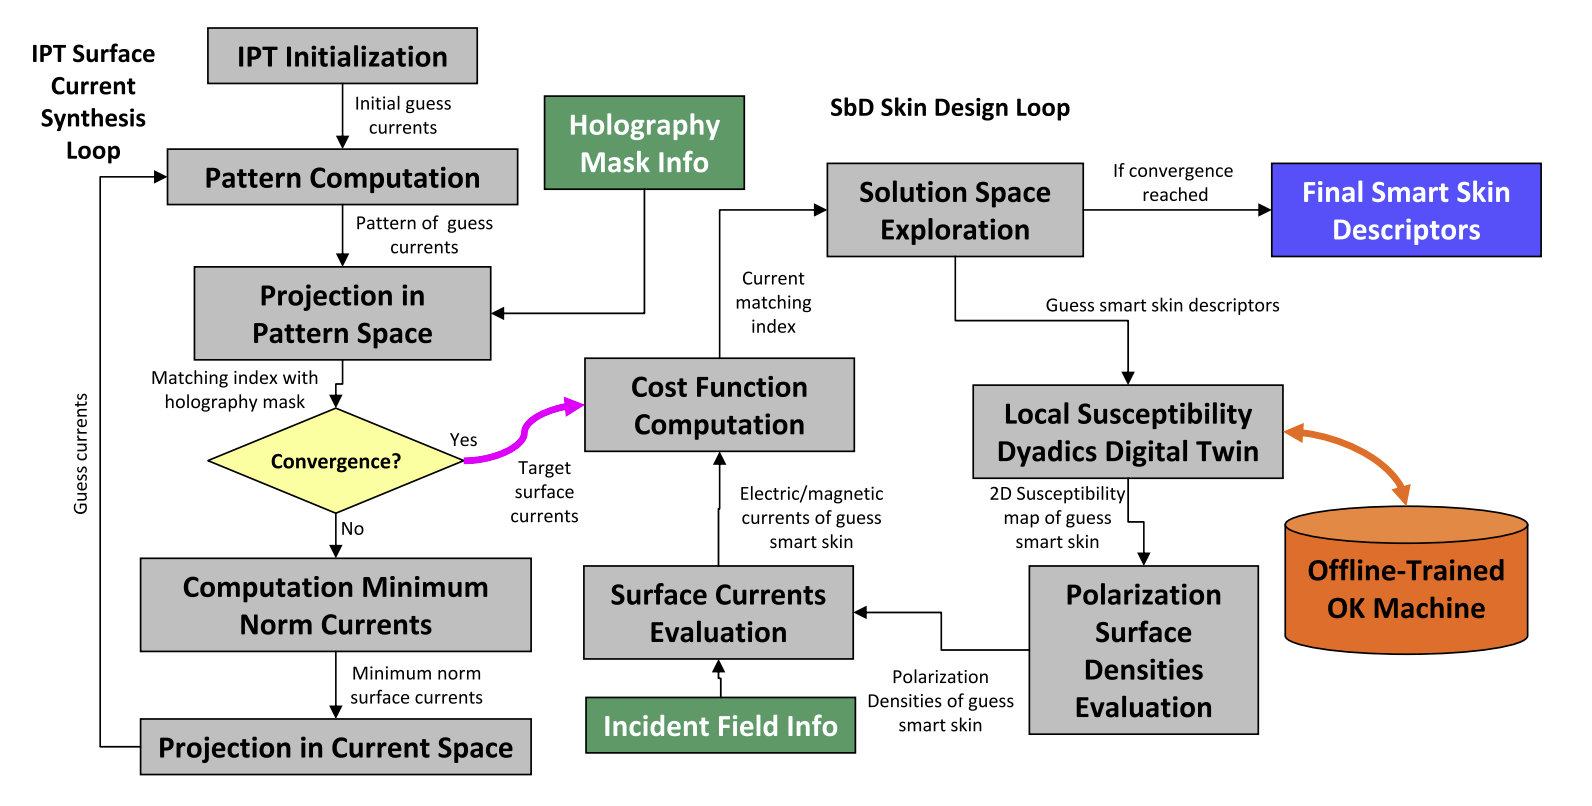
\includegraphics[%
  scale=0.3]{./Figure/Figure02.png}\end{center}


\caption{\footnotesize\label{cap:Design}SPSS Design Approach. Flowchart of the \emph{IPT-SbD}
holographic metasurface synthesis process with details of the elementary
blocks and their functional relations.}
\end{figure}


The problem formulated in \ref{sub:Mathematical-And-Design-Formulas}
needs a combination of \emph{ad-hoc} customized techniques to be solved.
In {[}Salucci.2018{]}(\cite{Salucci:2018}), is pointed out that the
\emph{IS} is affected by ill-posedness, caused by the nonuniqueness
of the radiation operator due to the existence of nonradiating currents,
which is a problem when the \emph{IS} is concerned with the synthesis
of the \emph{ideal} surface currents, $\{[\mathbf{J}^{w}(\mathbf{r})]^{*};w=\{ e,m\}\}$.
With that said, it's not doable to directly translate the design method
used in {[}Salucci.2018{]}(\cite{Salucci:2018}) to \emph{SPSS} case
since it purposely made for a {}``pattern matching objective'' and
not a {}``footprint pattern mask constrained'' one, such as the
one is considered. The need to consider a different solution strategy,
inspired by the \emph{IPT}, is absolute.

Firstly, needs to be defined the {}``pattern'' feasible space

\begin{equation}
\mathcal{F}\{[\mathbf{E}^{FF}(\mathbf{r})]^{*}\}\triangleq\{[\mathbf{E}^{FF}(\mathbf{r})]^{*}:\mathcal{L}(\mathbf{r})\leq|[\mathbf{E}^{FF}(\mathbf{r})]^{*}|^{2}\leq\mathcal{U}(\mathbf{r});\mathbf{r}\in\Xi\}\label{eq:18}\end{equation}


and the {}``current'' feasible space

\begin{equation}
\mathcal{F}\{[\mathbf{J}^{w}(\mathbf{r})]^{*}\}\triangleq\{[\mathbf{J}^{w}(\mathbf{r})]^{*}:[\mathbf{J}^{w}(\mathbf{r})]^{*}=C^{w}\exp[j\psi^{w}(\mathbf{r})];\mathbf{r}\in\Omega\}\label{eq:19}\end{equation}


where $C^{w}$ and $\psi^{w}(\mathbf{r})$ are, respectively, the
constant magnitude and profile of the locally-controlled phase of
the $w$-th $(w=\{ e,m\})$ current component.

Despite the fact that different scenarios and assumptions can be made
while defining the feasibility spaces aforementioned, the \ref{eq:19}
clearly implies that the \emph{SPSSs} unit cells do not allow a control
of the local magnitude of the electric/magnetic currents. Having done
all of the required assumption, we are able to implement the \emph{IPT-}based
design of the \emph{SPSS} currents design (\ref{cap:Design}) accordingly
to the following iterative procedure ($h=1,\cdots,H$ being the iteration
index) :

\begin{itemize}
\item \textbf{Initialization} (\emph{h=0}):\\
The $w$-th ($w=\{ e,m\}$) surface current is discretized\begin{equation}
\mathbf{J}_{h}^{w}(\mathbf{r})=\sum_{p=1}^{P}\sum_{q=1}^{Q}[(J_{h}^{w})_{x}^{pq}\mathbf{\hat{x}}+J_{h}^{w})_{y}^{pq}\mathbf{\hat{y}}]\Pi^{pq}(\mathbf{r})\label{eq:20}\end{equation}
\\
the expansion coefficients, $\{(J_{h}^{w})_{x}^{pq});p=1,\cdots,P;q=1,\cdots,Q\}$
and $\{(J_{h}^{w})_{y}^{pq};p=1,\cdots,P;q=1,\cdots,Q\}$ being set
to random values such that the condition $||(J_{h}^{w})_{x}^{pq}\mathbf{\hat{x}}+(J_{h}^{w})_{y}^{pq}\mathbf{\hat{y}}||=C^{w}(p=1,\cdots,P;q=1,\cdots,Q)$
holds true;
\item \textbf{Pattern Computation:}\\
The far-field pattern $\mathbf{E}_{h}^{FF}(\mathbf{r})$ is evaluated
in the coverage region $\Xi$ by substituting \ref{eq:20} in \ref{eq:4};
\item \textbf{Projection to Pattern Feasibility Space}:\\
The projected pattern $\mathbf{\tilde{E}}_{h}^{FF}(\mathbf{r})$ is
obtained by setting \begin{equation}
\left\{ \begin{array}{cc}
\sqrt{\mathcal{U}(\mathbf{r})} & if\,|\mathbf{E}_{h}^{FF}(\mathbf{r})|^{2}>\mathcal{U}(\mathbf{r})\\
\sqrt{\mathcal{L}(\mathbf{r})} & if\,|\mathbf{E}_{h}^{FF}(\mathbf{r})|^{2}<\mathcal{L}(\mathbf{r})\\
\mathbf{\mathbf{E}}_{h}^{FF}(\mathbf{r}) & otherwise\end{array}\right.\label{eq:21}\end{equation}

\item \textbf{Convergence Check}:\\
The algorithm is terminated by returning the ideal/reference $w$-th
($w=\{ e,m\}$) surface current, $[\mathbf{J}^{w}(\mathbf{r})]^{*}=\mathbf{J}_{h}^{w}(\mathbf{r})$,
if $h=H$ or the \emph{pattern matching index}, $\chi_{h}$,\begin{equation}
\chi_{h}=\frac{\int_{\Xi}|\mathbf{\tilde{E}}_{h}^{FF}(\mathbf{r})-\mathbf{E}_{h}^{FF}(\mathbf{r})|^{2}d\mathbf{r}}{\int_{\Xi}|\mathbf{E}_{h}^{FF}(\mathbf{r})|^{2}d\mathbf{r}}\label{eq:22}\end{equation}
\\
satisfies the condition $\chi_{h}\leq\chi^{*},\chi^{*}$ being a user-chosen
convergence threshold;
\item \textbf{Computation of Minimum Norm Currents}:\\
Compute the \emph{minimum norm} component of the $w$-th ($w=\{ e,m\}$)
surface current, $[\mathbf{J}_{h}^{w}(\mathbf{r})]^{MN}$ (MN means
\emph{minimum norm}), by solving \ref{eq:4} with respect to the currents.
Towards this end, the method based on the truncated singular value
decomposition, detailed in {[}Salucci.2018{]}(\cite{Salucci:2018}),
is applied;
\end{itemize}
\textbf{Projection to Current Feasibility Space:}\\
Update the iteration index $(h\leftarrow h+1)$ and evaluate the $w$-th
$w=\{ e,m\}$ projected surface current $\mathbf{J}_{h}^{w}(\mathbf{r})$\begin{equation}
\mathbf{J}_{h}^{w}(\mathbf{r})=C^{w}\times\sum_{p=1}^{P}\sum_{q=1}^{Q}\frac{[(J_{h-1}^{w})_{x}^{pq}]^{MN}\mathbf{\hat{x}}+[(J_{h-1}^{w})_{y}^{pq}]^{MN}\mathbf{\hat{y}}}{||[(J_{h-1}^{w})_{x}^{pq}]^{MN}\mathbf{\hat{x}}+[(J_{h-1}^{w})_{y}^{pq}]^{MN}\mathbf{\hat{y}}||}\Pi^{pq}(\mathbf{r})\label{eq:23}\end{equation}
\\
Restart process from the \textbf{{}``Pattern Computation''} step.\\
Once the referecne surface currents, $\{[\mathbf{J}^{w}(\mathbf{r})]^{*};w=\{ e,m\}\}$,
have been found, the \emph{Sub-problem 2} is then adressed by solving
\ref{eq:16}. More precisely, an iterative \emph{SbD-}based strategy
inspired is customized to the problem at hand by implementing the
following blocks of the functional flowchart in \ref{cap:Design}:

\begin{enumerate}
\item the {}``Solution Space Exploration (\emph{SSE})'' block aimed at
optimizing the \emph{SPSS} descriptors by defining a succession of
\emph{S} iterations (\emph{s} being the \emph{SbD} iteration index,
$s=1,\cdots,S$) where \emph{G} trial solutions, $\{\mathcal{D}_{g}^{(s)};g=1,\cdots,G\}$,$\mathcal{D}_{g}^{(s)}\triangleq\{\mathbf{d}_{pq}|_{g}^{(s)};p=1,\cdots,P;q=1,\cdots,Q\}$
being the $g$-th trial at the $s$-th iteration, evolve towards the
global solution $\mathcal{D}^{opt}$\ref{eq:16}. As said before,
being the nature of the problem at hand ill-posed, and considering
the non-linear function to be optimized, a global search mechanism
based on the \emph{Particle Swarm Optimizer (PSO)}%
\footnote{PSO method%
}{\let\thefootnote\relax\footnotetext{Is a computational method that optimizes a problem byt iteratively trying to improve a candidate solution iwth regard to a given measure of quality}}
has been chosen to update/evolve the population of trial solutions
at each $s$-th ($s=1,\cdots,S$) step, $\mathcal{D}^{(s)}$;
\item the {}``Cost Function'' (\emph{CF}) evaluation block that implements
the discretized version of \ref{eq:16};
\item the {}``Surface Current Evaluation'' (\emph{SCE}) block that employs
\ref{eq:5} and \ref{eq:6} to determine $\mathbf{J}^{w}(\mathbf{r})$
starting from $\mathbf{B}^{w}(\mathbf{r}),w=\{ e,m\}$;
\item the {}``Polarization Surface Densities Evaluation'' (\emph{PSDE})
block that implements \ref{eq:7} and \ref{eq:8} to yield the $w$-th
($w=\{ e,m\}$) polarization surface density, $\mathbf{B}^{w}(\mathbf{r})$;
\item the {}``Local Susceptibility Dyadics Digital Twin'' (\emph{LSDDT})
block devoted to determine $\overline{\overline{\chi}}(\mathbf{d}_{pq}|_{g}^{(s)})$
and $\overline{\overline{\xi}}(\mathbf{d}_{pq}|_{g}^{(s)})$ to be
used in the \emph{PSDE} block to compute the polarization surface
densities at each $s$-th $(s=1,\cdots,S)$ iteration for each $g$-th
($g=1,\cdots,G$) guess solution in each $(p,q)$-th ($p=1,\cdots,P;q=1,\cdots,Q$)
unit cell of the \emph{SPSS. }
\end{enumerate}
As for the last point treated and analogously to the unit cell of
reflectarrays, each susceptibility tensor set, $\overline{\overline{\chi}}(\mathbf{d}_{pq}|_{g}^{(s)})$
and $\overline{\overline{\xi}}(\mathbf{d}_{pq}|_{g}^{(s)})$, generated
in the \emph{SbD} iterative process, is full-wave evalueted; the result
is computationally unfeasible, since this would require the numerical
modelling and the full-wave solution of $P\times Q\times G\times S$
\emph{SPSSs.} With that said, the dyadics, $\overline{\overline{\chi}}(\mathbf{d})$
and $\overline{\overline{\xi}}(\mathbf{d})$, are approximated with
their surrogate $\overline{\overline{\chi}}^{\prime}(\mathbf{d})$
and $\overline{\overline{\xi}}^{\prime}(\mathbf{d})$, as the (\emph{DT})
states, which is implemented according to a statistical learning approach
based on the \emph{Ordinary Kringing (OK)}%
\footnote{OK Method%
}{\let\thefootnote\relax\footnotetext{Is a spatial estimation method where the error variance is minimized. It's not dependent on the data usedto make the estimate.}}
\emph{}method starting from a set of $A$ full-wave computed unit
cell responses $[\mathbf{d}_{a};\overline{\overline{\chi}}(\mathbf{d}_{a});\overline{\overline{\xi}}(\mathbf{d}_{a})],a=1,\cdots,A$.
Since the \emph{OK} is capable of effectively creating reliable and
accurate surrogate models of wave manipulating devices , its choice
is obvious. 

Since, in {[}Yang.2021{]}(\cite{Yang:2021}) has been computed $\overline{\overline{\chi}}(\mathbf{d}_{a}),\overline{\xi}(\mathbf{d}_{a})$,
starting from the full-wave simulation of the unit cell reflection
matrix under local periodicity assumption $\overline{\overline{\Gamma}}(\mathbf{d}_{a})$
and retrieving the associated dyadics by standard inversion formulas
such as\begin{equation}
\xi_{xx}(\mathbf{d}_{a})=\frac{2j}{k_{0}}\frac{\Gamma_{\perp\perp}(\mathbf{d}_{a})+1}{\Gamma_{\perp\perp}(\mathbf{d}_{a})-1}\label{eq:24}\end{equation}


which is valid for reflecting cells (in {[}Yang.2021{]}(\cite{Yang:2021}),
Chapter 3, the author has computed this application on other components).

It is worth considering the fact that the \emph{DT} has to predict
the local susceptibility tensor rather than the local reflection coefficient,
since the reflectarray case is not experimented. This means that 6
complex coefficients (adding $\overline{\overline{\chi}}(\mathbf{d})$
and $\overline{\overline{\xi}}(\mathbf{d})$ to the count) are computed,
instead of 4 terms, deriving from the reflection matrix. This implies
that the \emph{DT} of a \emph{SPSS} can neglect the incidence angle
of the illuminating field since the susceptibility tensor does not
depend on it, unlike what has been treated in {[}Yang.2021{]}\cite{Yang:2021}.

Since have been treated all the aspects of the \emph{IPT-SbD} flowchart,
a numerical experimentation will follow this section, considering
various footprints, since, as said before, our problem takes in account
a {}``footprint pattern mask'' costraint.
\subsection{Numerical Results\label{sub:Numerical-Results}}

Since the formulation of all the needed formulas, criterias and procedures,
has been done, the next step is to numerically resolve the \emph{Sub-Problem
1} and \emph{Sub-Problem 2,} besides the value of the pattern matching
index of the \emph{SPSS} final layout, $\mathcal{X}$ \ref{eq:22}
\emph{},utilizing all the data contained in \ref{cap:Data}%
\footnote{Computational Times%
}{\let\thefootnote\relax\footnotetext{The computational times refer to non-optimized MATLAB serial implementaions exectued on a single-core laptop running at $1.60 \, [GHz]$.}}.
The data found in \ref{cap:Data} are quantified by computing the
\emph{reference pattern matching} $\mathcal{X}^{IPT}$ ($\mathcal{X}^{IPT}\triangleq\mathcal{X}_{H}$,
referenced in \emph{Sub-Problem 1}) and the \emph{surface current
fidelity index $v^{SbD}$} ($v^{SbD}\triangleq v(\mathbf{J}^{w}(\mathbf{r})|_{s=S};[\mathbf{J}^{w}(\mathbf{r})]^{*}$,
referenced in \emph{Sub-Problem 2}). The focus of this section is
to prove the effectiveness, through the illustration of the \emph{IPT-SbD}
design process, for the synthesis of footprint pattern shaped holographic
\emph{SPSSs. }

\begin{center}%
\begin{table}[H]
\begin{center}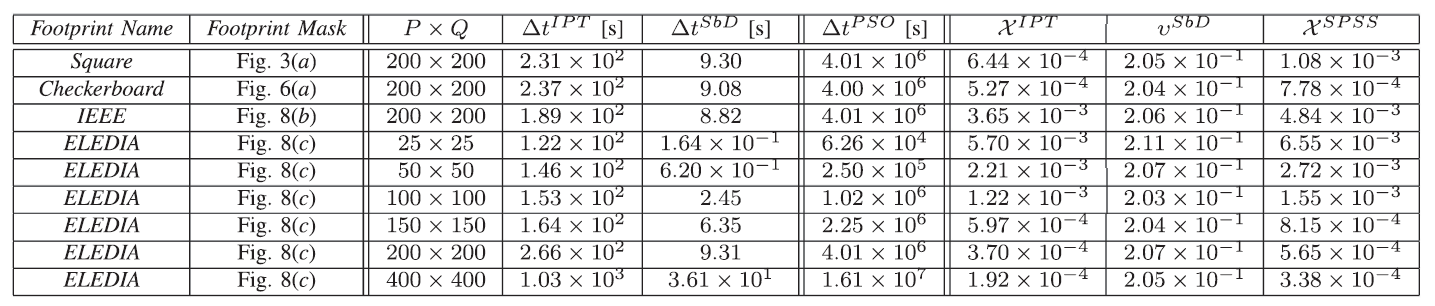
\includegraphics[scale=0.5]{./Figure/FIgure03.png}\end{center}
\caption{\footnotesize\label{cap:Data}Numerical Validation, Matching and Computational
Indexes }
\end{table}
\end{center}

The benchmark SEE scenario is modeled after this features:

\begin{itemize}
\item Base Station that illuminates from $(\theta^{inc},\varphi^{inc})=(20,105)[\deg]$;
\item Linearly-Polarized plane wave with a $+45[\deg]$ slant polarization
at $f=30[GHz]$
\item Different \emph{SPSS} apertures and target footprint masks
\item The metasurface unit cell, which consists of a square passive and
static metallic patch, with periodicity $\delta_{x}=\delta_{y}=5.0\times10^{-3}[m]$
, printed on a single-layer substrate (Rogers 3003 dielectrict with
thickness $\tau=5.08\times10^{-4}[m]$) has been used ($L=1$) and
modelled in \emph{HFSS} for generating/training the \emph{LSDDT} block.\\
A simple yet efficient structure has been chosen to highlight the
potentials of the \emph{IPT-SbD} strategy, even when dealing with
elementary unit cells which feature an inexpensive fabrication process
since: only one dielectric layer is employed, the metalization contour
complexity is very limited and no via holes are present;
\item The following \emph{IPT-SbD} based parameters has been chosen %
\footnote{\cite{Yang:2021}%
}{\let\thefootnote\relax\footnotetext{As stated in [Yang.2021] (and in all citated papers inside), the following parameters has been chosen through \textit{deterministic and stochastic} optimization techniques.}}:
$H=10^{3},\mathcal{X}^{*}=10^{-4},S=10^{4}$ and $G=10$.
\end{itemize}

\subsubsection{{}``Square'' Footprint Experiment}

%
\begin{figure}[H]
\begin{center}\begin{tabular}{cc}
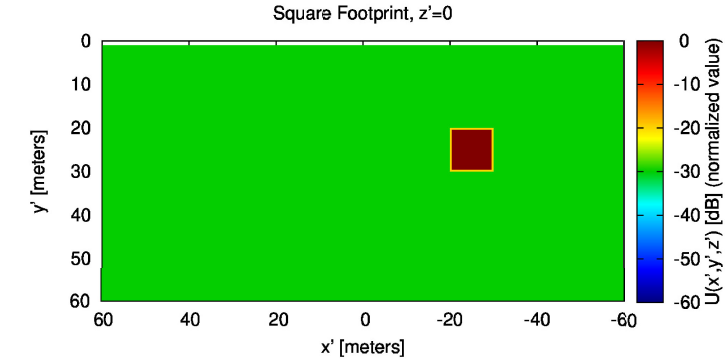
\includegraphics[%
  scale=0.35]{./Figure/Figure04.png}&
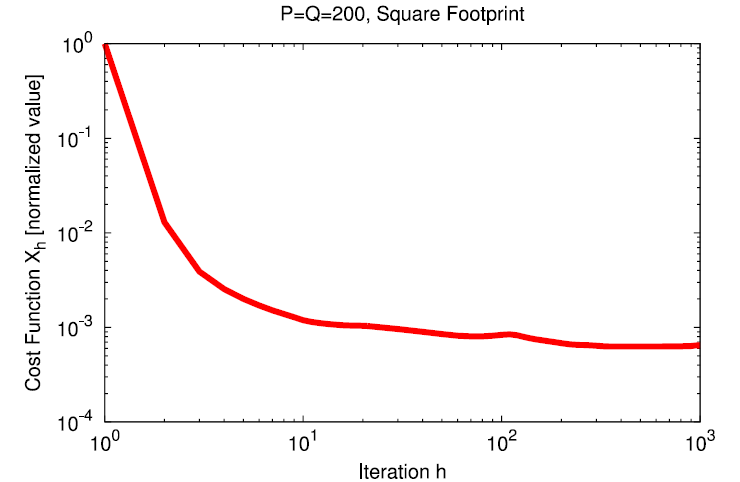
\includegraphics[%
  scale=0.35]{./Figure/Figure05.png}\tabularnewline
(a)&
(b)\tabularnewline
\end{tabular}\end{center}


\caption{\footnotesize\label{cap:Square_Image}Numerical Validation (\emph{{}``Square''}
\emph{Footprint, $P=Q=200$}) - Plot of (a) the footprint pattern
mask $[\mathcal{U}(\mathbf{r}^{\prime});\mathbf{r^{\prime}}\in\Theta]$
and (b) evolution of the \emph{IPT} cost function versus the iteration
index, $h(h=1,\cdots,H)$.}
\end{figure}


The first proposed fooprint pattern is a $P\times Q=200\times200$
holographic \emph{SPSS} with an $1\times1[m]$ support $\Omega$,
as explained in \ref{cap:Geom}, located at the position $(x^{\prime},y^{\prime},z^{\prime})=(0,0,15)[m]$
in the global coordinate system. The upper and lower masks have been
defined so that the skin reflect a constant-power square footprint
in the coverage region $\Xi$ of lateral size $10[m]$ centered at
$(x^{\prime},y^{\prime},z^{\prime})=(-25,25,0)[m]$ {[}''Square Footprint''
- \ref{cap:Square_Image}(a){]}, while a $-30[dB]$ footprint power
reduction has been enforcer outside $\Xi$ in the observation region
$\Theta$of extension $120\times60[m^{2}]$. 

As seen in \ref{cap:Square_Image}(b), the evolution on the \emph{IPT}
cost function (modelled after the steps solved in the \emph{IPT-}based
iterative procedure in \ref{sub:Synthesis-Procedure}), there is a
quick minimization and a convergence to a solution with a very small
mismatch from the target footprint pattern, $\mathcal{X}_{H}=6.44\times10^{-4}$
in less than 4 minutes \ref{cap:Data} thanks to the exploitation
of a fast Fourier transformarm within the \emph{IPT} loop despite
the huge number of unknowns.

%
\begin{figure}[H]
\noindent \begin{center}\begin{tabular}{cc}
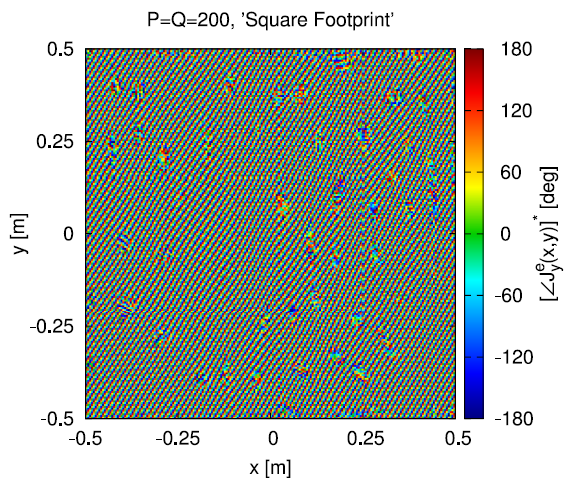
\includegraphics[%
  scale=0.35]{./Figure/FIgure06.png}&
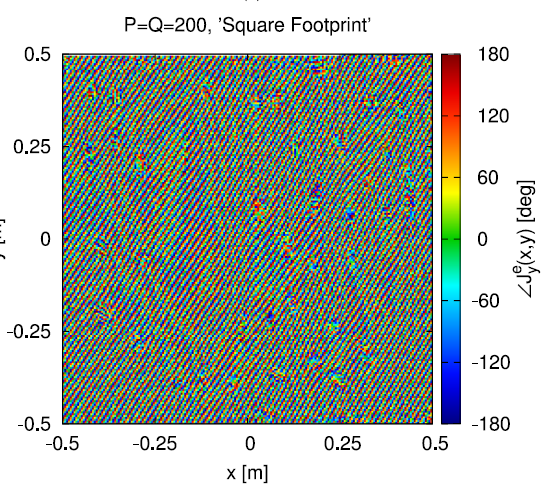
\includegraphics[%
  scale=0.35]{./Figure/Figure07.png}\tabularnewline
(a)&
(b)\tabularnewline
\multicolumn{2}{c}{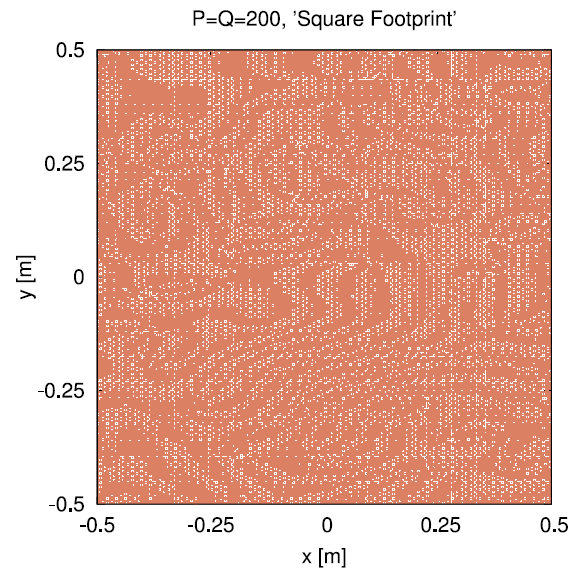
\includegraphics[%
  scale=0.35]{./Figure/Figure08.png}}\tabularnewline
\multicolumn{2}{c}{(c)}\tabularnewline
\end{tabular}\end{center}


\caption{\footnotesize\label{cap:Square_Phase} Numerical Validation (\emph{{}``Square''}
\emph{Footprint, $P=Q=200$}) - Plot of the phase distribution of
(a) the \emph{IPT-}reference/ideal current along with (b) that generated
by the synthesized \emph{SPSS} layout (c).}
\end{figure}


%
\begin{figure}[H]
\begin{center}\begin{tabular}{cc}
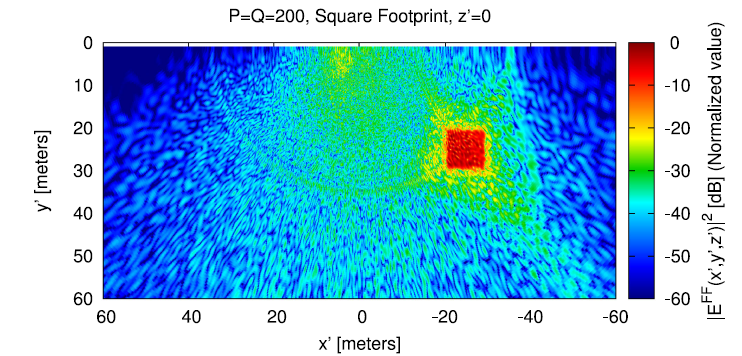
\includegraphics[%
  scale=0.4]{./Figure/Figure09.png}&
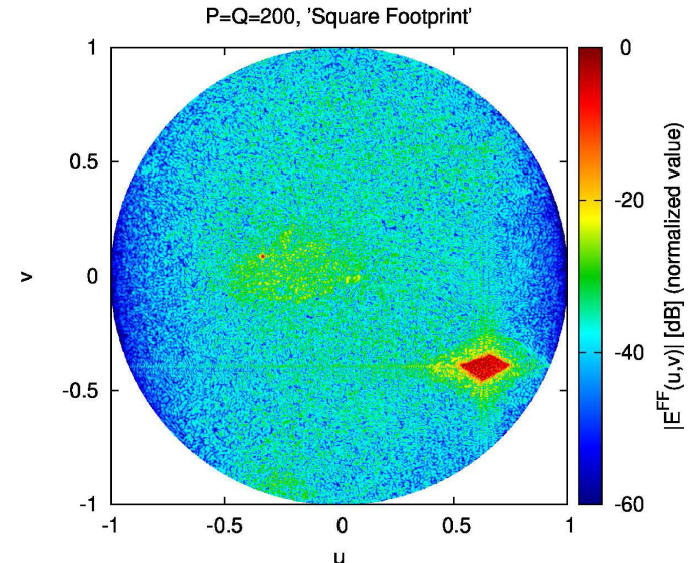
\includegraphics[%
  scale=0.4]{./Figure/FIgure10.png}\tabularnewline
(a)&
(b)\tabularnewline
\end{tabular}\end{center}


\caption{\footnotesize\label{cap:Square_Radiation}Numerical Validation (\emph{{}``Square''}
\emph{Footprint, $P=Q=200$}) - Plots of the radiated (a) footprint
pattern within the observation region $\Theta$ and (b) angular power
distribution. }
\end{figure}


Proceeding to the \emph{Sub-Problem 2,} the \emph{SbD} optimization
process quickly ($\Delta t^{SbD}<10[s]$ - \ref{cap:Data}) yields,
thanks to an accurate matching with the reference current {[}\ref{cap:Square_Phase}(a)
vs. \ref{cap:Square_Phase}(b){]}, a final layout {[}\ref{cap:Square_Phase}(c){]}
that faithfully fulfills the mask requirements as pictorially confirmed
by the plot of the radiated footprint pattern within the observation
region {[}\ref{cap:Square_Radiation}(a) vs. \ref{cap:Square_Image}(a){]}
.

As seen from the data in \ref{cap:Data}, the time using the \emph{IPT-}based
process versus the time using the \emph{PSO-}driven optimization in
significantly lower {[}$\Delta t^{IPT}$ vs. $\Delta t^{PSO}$ {]},
remarking the efficiency of the synthesis procedure detailed in \ref{sub:Synthesis-Procedure}.

Another point worth noting is the {}``focusing'' skill of the \emph{SPSS}
seen in \ref{cap:Square_Radiation}(c): as seen, the synthesized \emph{SPSS}
has the ability to compensate the angular beam distorsion caused by
the position and the orientation of the coverage region, with respect
to the smart skin and the incident wave. As expected, in a real-life
environment, it's crucial for the smart skin to be able to compensate
such error, otherwise the need for the \emph{IPT-SbD} based process
it's unnecessary. This will expanded further in the \ref{sec:Olivieri.2021-Conclusions}
section, with reference to all other experiments.


\subsubsection{{}``Checkerboard'', {}``IEEE'' and {}``ELEDIA'' Footprint Experiment}

%
\begin{figure}[H]
\begin{center}\begin{tabular}{cc}
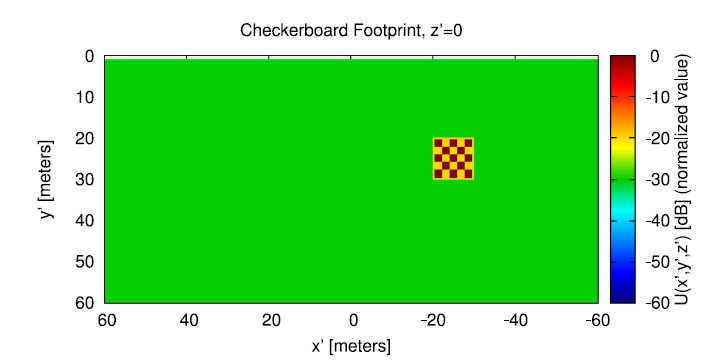
\includegraphics[%
  scale=0.35]{./Figure/Figure11.png}&
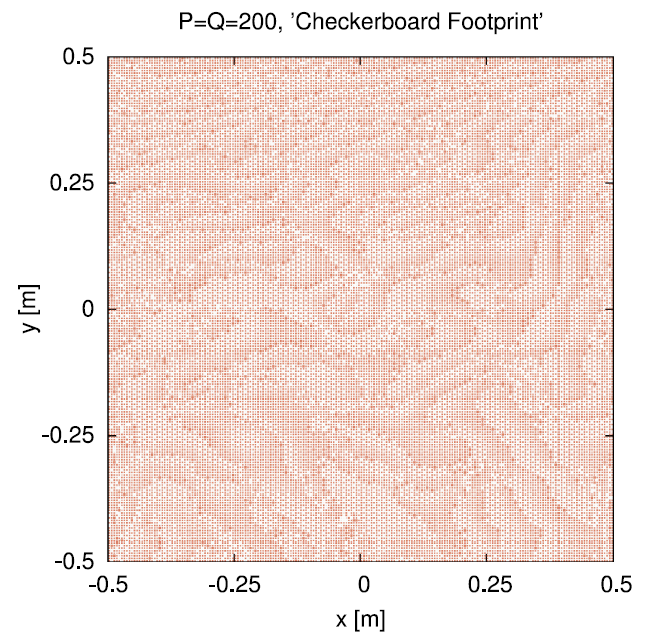
\includegraphics[%
  scale=0.35]{./Figure/Figure12.png}\tabularnewline
(a)&
(b)\tabularnewline
\end{tabular}\end{center}


\caption{\footnotesize\label{cap:Checkerboard_Image1}Numerical Validation (\emph{{}``Checkerboard''}
\emph{Footprint, $P=Q=200$}) - Plot of (a) the footprint pattern
mask $[\mathcal{U}(\mathbf{r}^{\prime});\mathbf{r^{\prime}}\in\Theta]$
and (b) layout of the synthesized \emph{SPSS.}}
\end{figure}


%
\begin{figure}[H]
\begin{center}\begin{tabular}{cc}
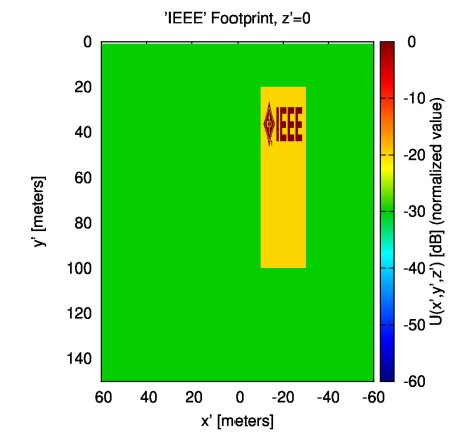
\includegraphics[%
  scale=0.35]{./Figure/Figure16.jpg}&
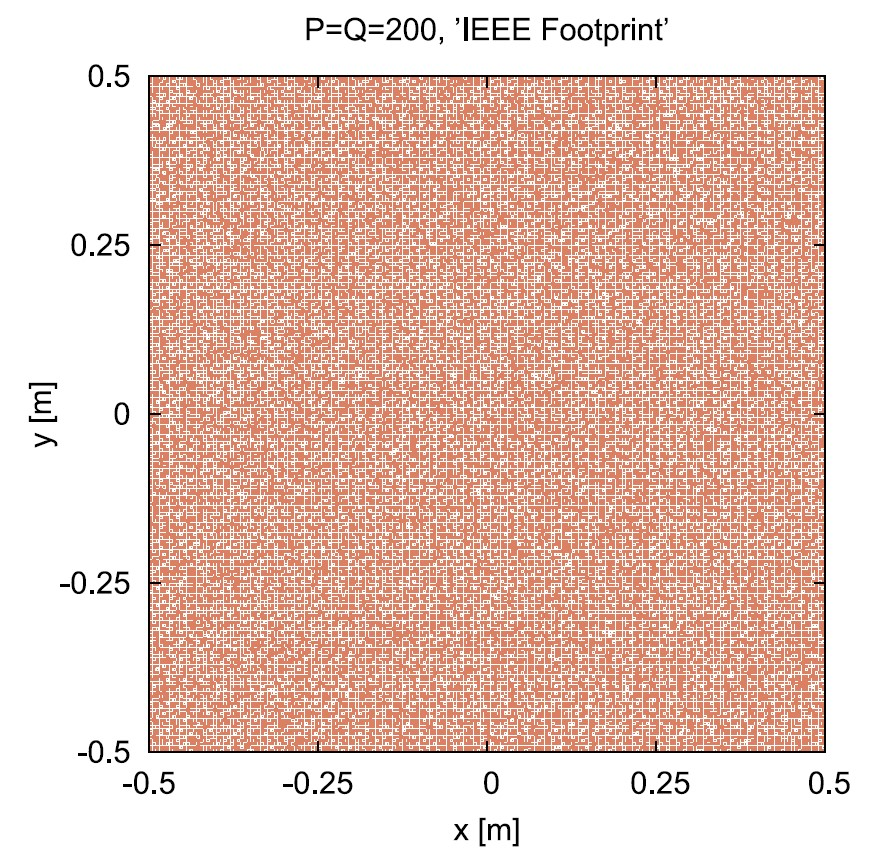
\includegraphics[%
  scale=0.3]{./Figure/Figure18.jpg}\tabularnewline
(a)&
(b)\tabularnewline
\end{tabular}\end{center}


\caption{\footnotesize\label{cap:IEEE_Image1}Numerical Validation (\emph{{}``IEEE''}
\emph{Footprint, $P=Q=200$}) - Plot of (a) the footprint pattern
mask $[\mathcal{U}(\mathbf{r}^{\prime});\mathbf{r^{\prime}}\in\Theta]$
and (b) layout of the synthesized \emph{SPSS.}}
\end{figure}


%
\begin{figure}[H]
\begin{center}\begin{tabular}{c}
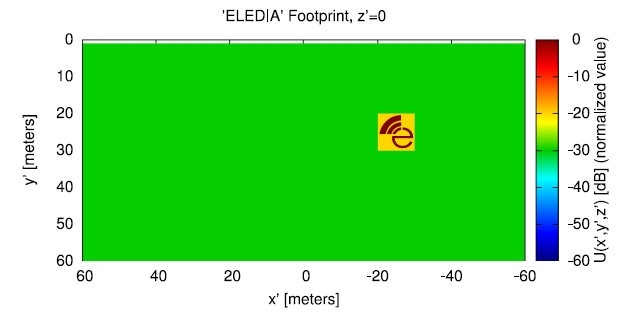
\includegraphics[%
  scale=0.35]{./Figure/Figure17.jpg}\tabularnewline
(b)\tabularnewline
\end{tabular}\end{center}


\caption{\footnotesize\label{cap:Checkerboard_Image2}Numerical Validation (\emph{{}``ELEDIA''}
\emph{Footprint, $P=Q$} have various values) - Plot of (a) the footprint
pattern mask $[\mathcal{U}(\mathbf{r}^{\prime});\mathbf{r^{\prime}}\in\Theta]$.}
\end{figure}


As seen, the footprint mask just show are more complex than the one
before. But, is worth nothing that the change in complexity of the
footprint masks don't impact on the \emph{CPU} time for synthesis
process nor on the convergence of the two-step synthesis. Taking in
example the {}``Checkerboard'' footprint, the difference is shown
as follows in Table (\ref{cap:Difference}):

%
\begin{table}[H]
\begin{center}\begin{tabular}{|c|c|c|}
\hline 
&
{}``Square''&
{}``Checkerboard''\tabularnewline
\hline
\hline 
$\Delta t^{IPT}[s]$&
$2.31\times10^{2}$&
$2.37\times10^{2}$\tabularnewline
\hline 
$\Delta t^{SbD}[s]$&
$9.30$&
$9.08$\tabularnewline
\hline 
$\mathcal{X}^{SPSS}$&
$1.08\times10^{-3}$&
$7.78\times10^{-4}$\tabularnewline
\hline
$v^{SbD}$&
$2.05\times10^{-1}$&
$2.04\times10^{-1}$\tabularnewline
\hline
\end{tabular}\end{center}


\caption{\footnotesize\label{cap:Difference}Computational difference between footprints}
\end{table}


As can be seen in the \ref{cap:IEEE_Image1}, it's worth noting for
the sake of the experiment, that even a complex-built footprint mask
can be used and perform in a matter of real-life utilization; the
pattern can be seen in Table\ref{cap:Table1}:

%
\begin{figure}[H]
\begin{center}\begin{tabular}{cc}
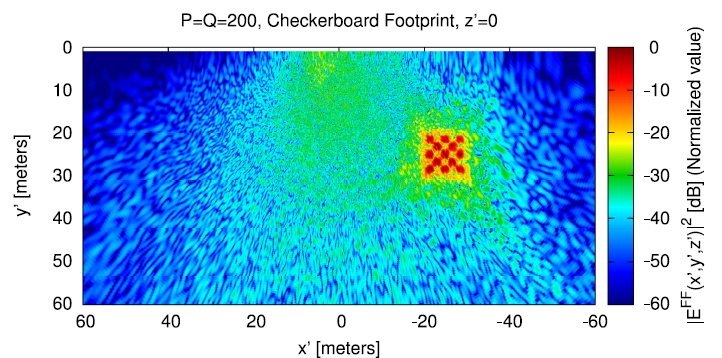
\includegraphics[%
  scale=0.4]{./Figure/Figure13.png}&
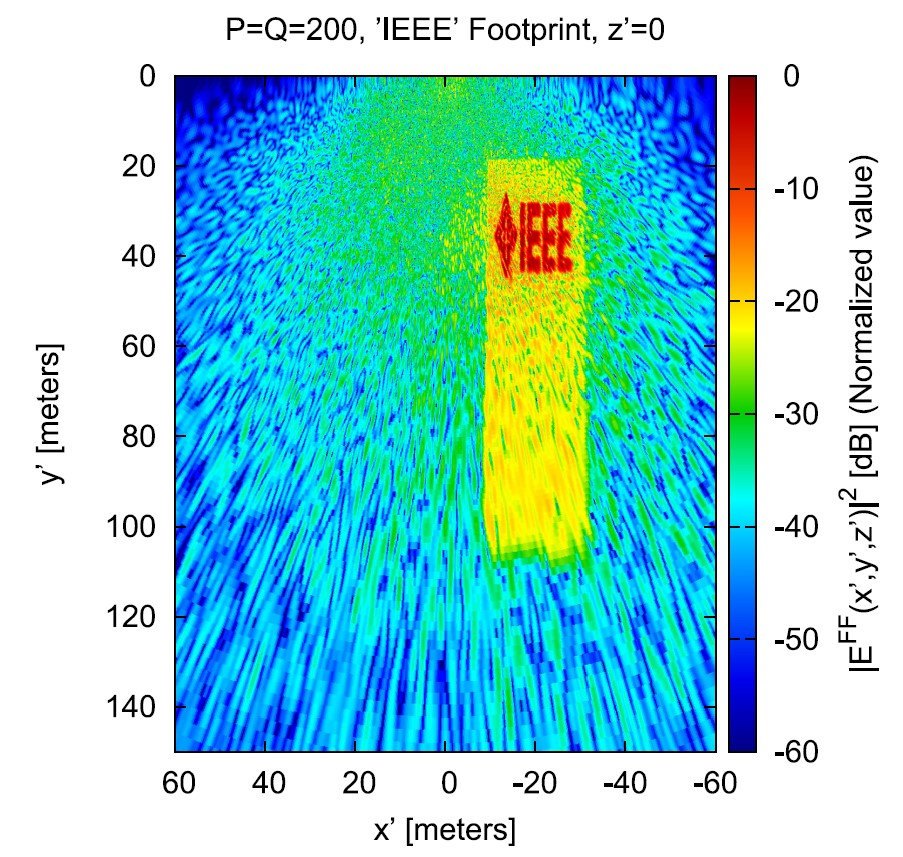
\includegraphics[%
  scale=0.3]{./Figure/Figure19.jpg}\tabularnewline
(a)&
(b)\tabularnewline
\end{tabular}\end{center}


\caption{\footnotesize\label{cap:Table1}Numerical Validation (\emph{{}``Checkerboard''}
and \emph{{}``IEEE''} \emph{Footprint, $P=Q=200$}) - Plots of the
radiated (a) {}``Checkerboard'' footprint pattern and (b) {}``IEEE''
footprint pattern within the observation region $\Theta$.}
\end{figure}


The {}``IEEE'' footprint pattern is modeled with a rectangle of
$20\times80[m]$ in front of the smart skin, which increases the local-complexity
of the footprint. 

Until now, it's been experimented with {}``fixed'' dimension masks;
but there is the need to verify if the \emph{IPT-SbD} process for
various mask dimensions. 

This experiment is going to be verified by introducing an {}``ELEDIA''
footprint mask, with dimensions varying from $P=Q=50$ to $P=Q=400$.

%
\begin{figure}[H]
\begin{center}\begin{longtable}{ccc}
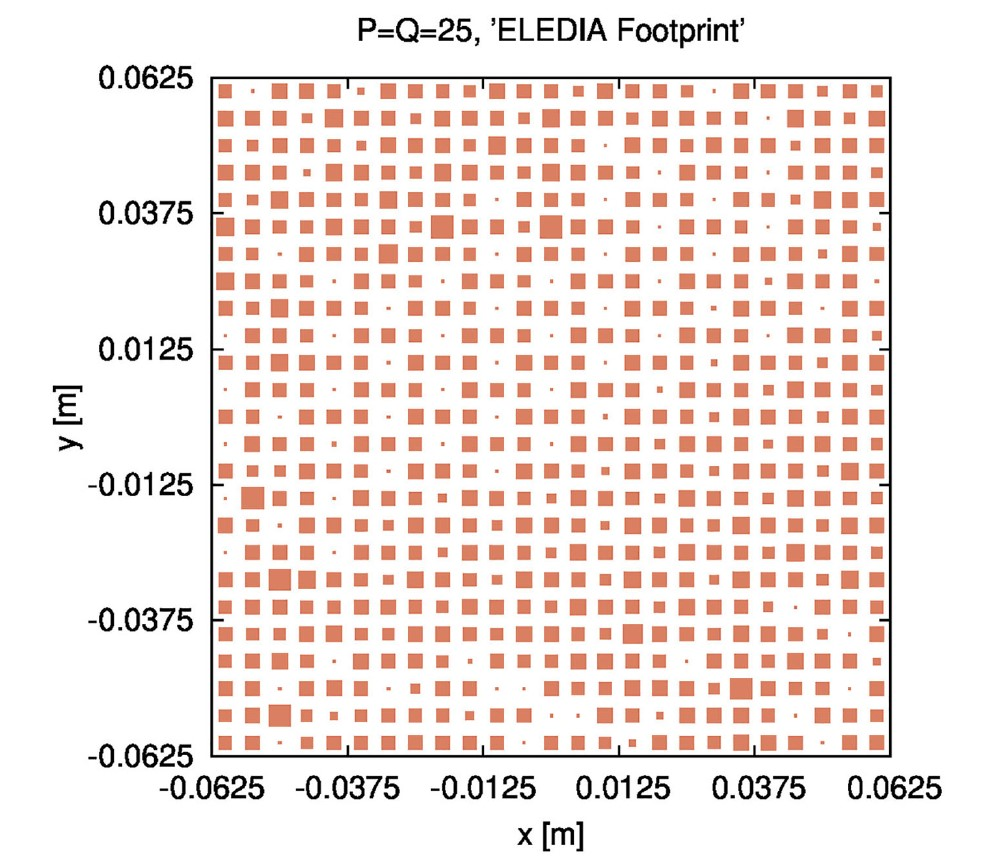
\includegraphics[scale=0.15]{./Figure/Figure20.jpg}&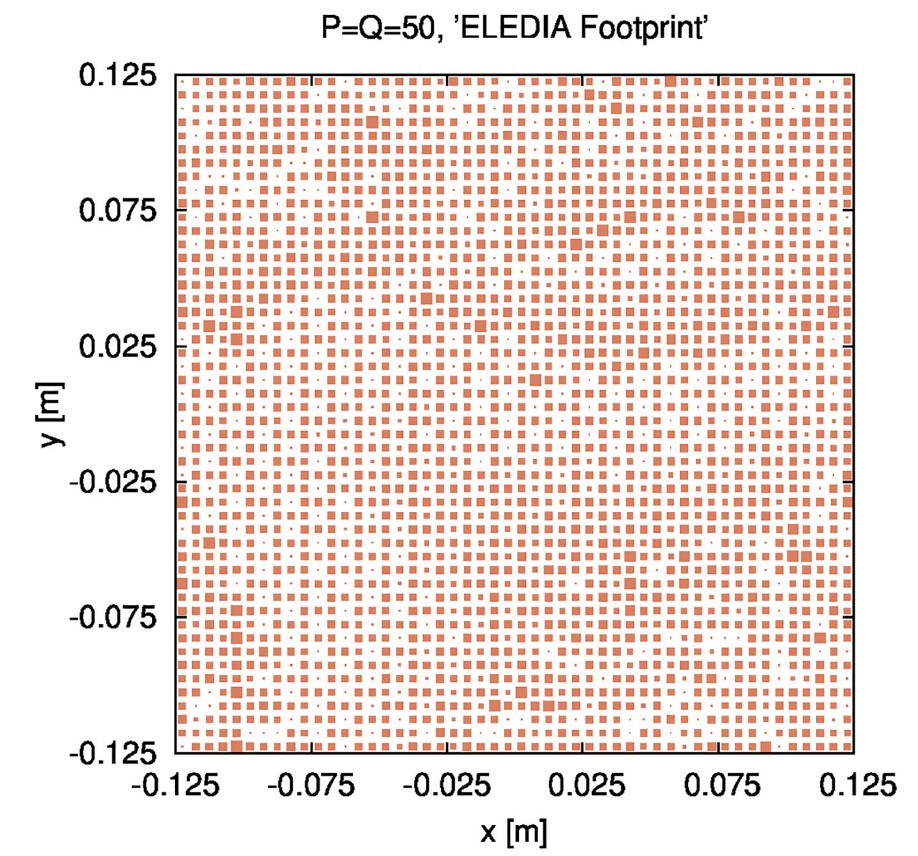
\includegraphics[scale=0.15]{./Figure/Figure21.jpg}&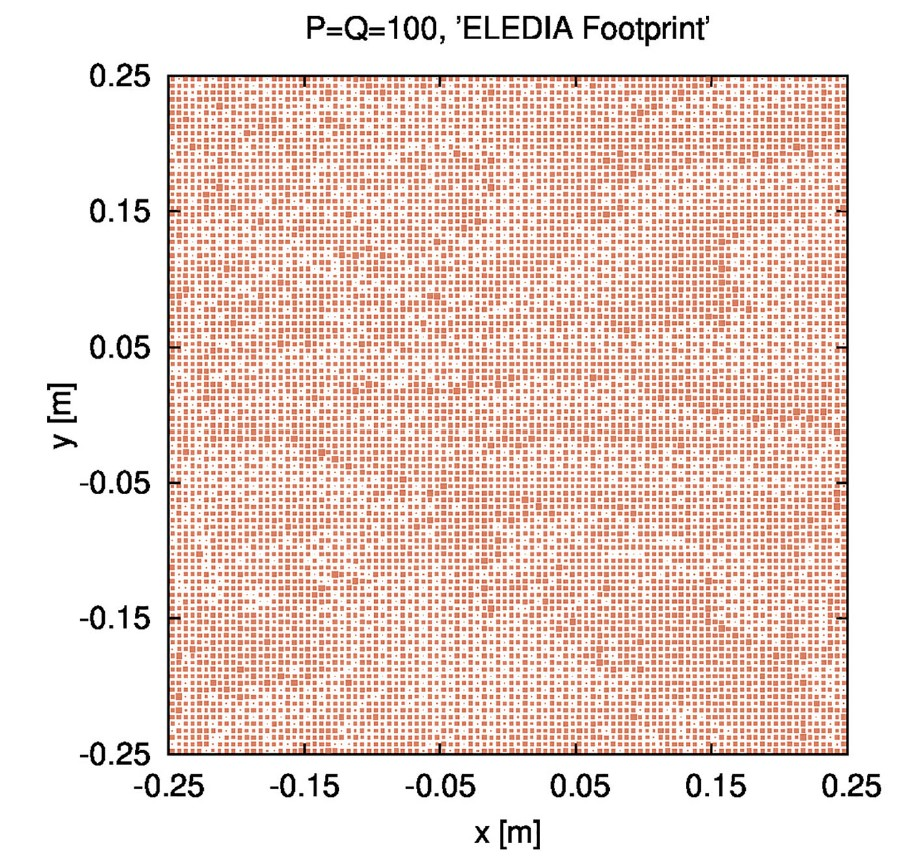
\includegraphics[scale=0.15]{./Figure/Figure22.jpg}\tabularnewline
(a)&(b)&(c)\tabularnewline
\newpage
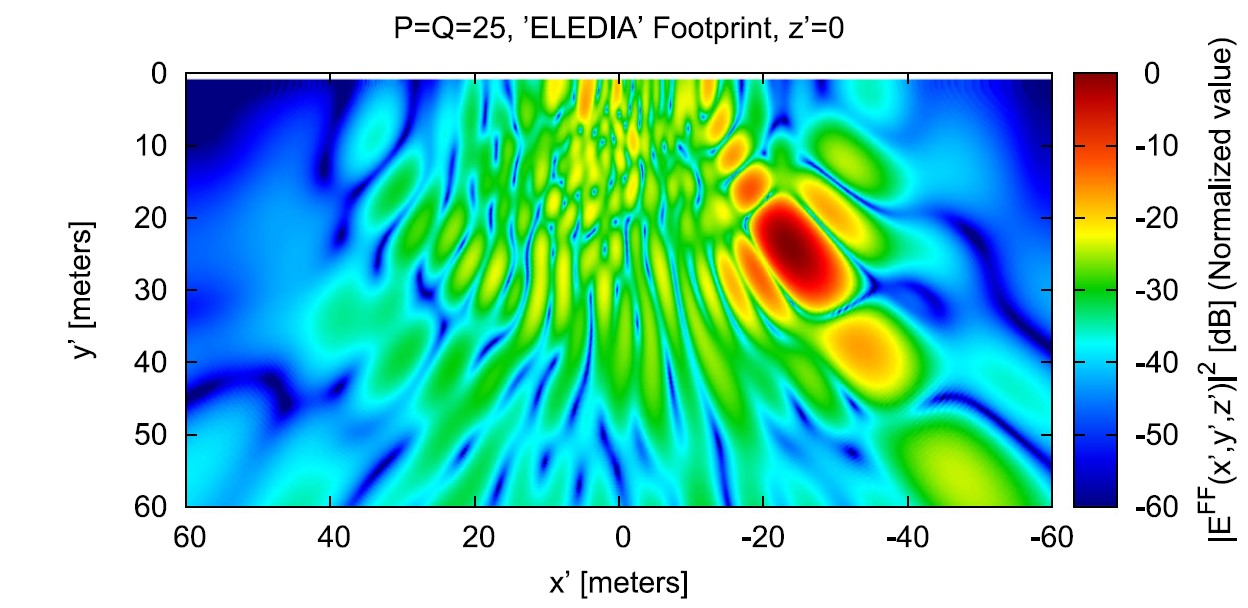
\includegraphics[scale=0.15]{./Figure/Figure26.jpg}&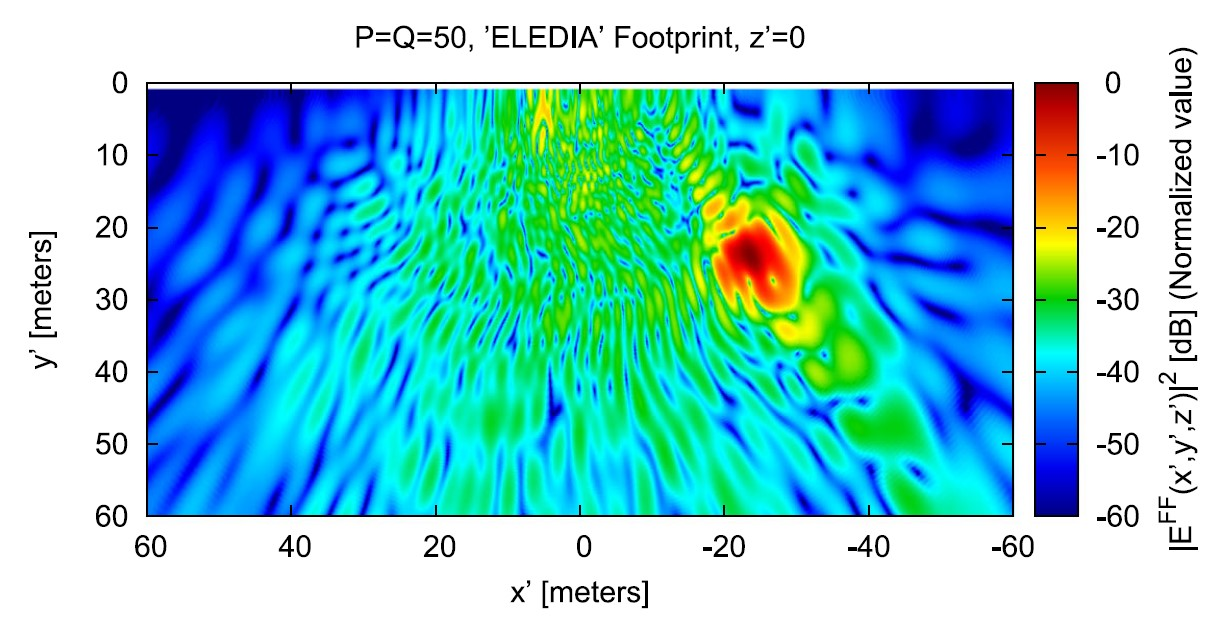
\includegraphics[scale=0.15]{./Figure/Figure27.jpg}&\includegraphics[scale=0.15]{./Figure/Figure28.jpg}\tabularnewline
(d)&(e)&(f)\tabularnewline
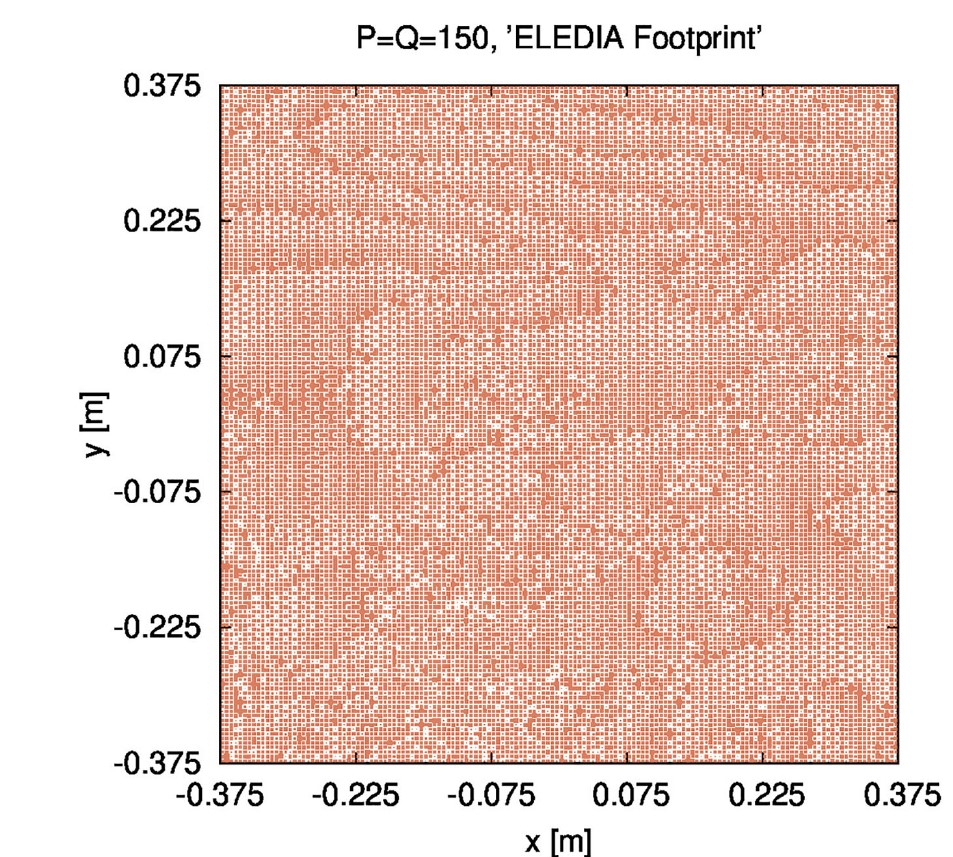
\includegraphics[scale=0.15]{./Figure/Figure23.jpg}&
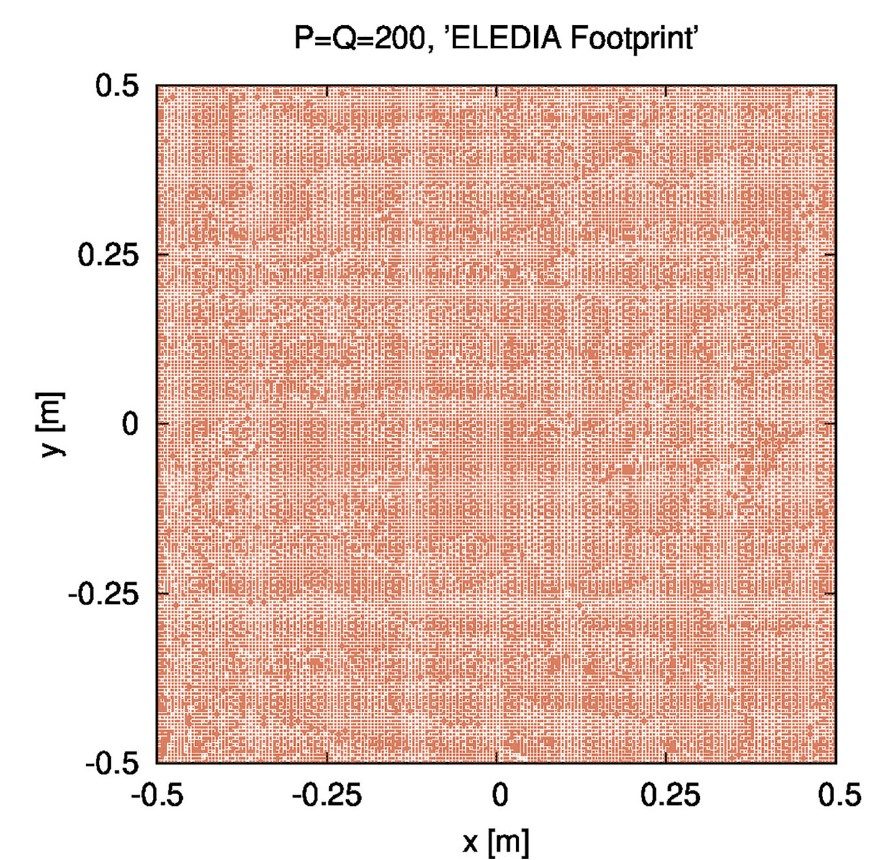
\includegraphics[scale=0.15]{./Figure/Figure24.jpg}&
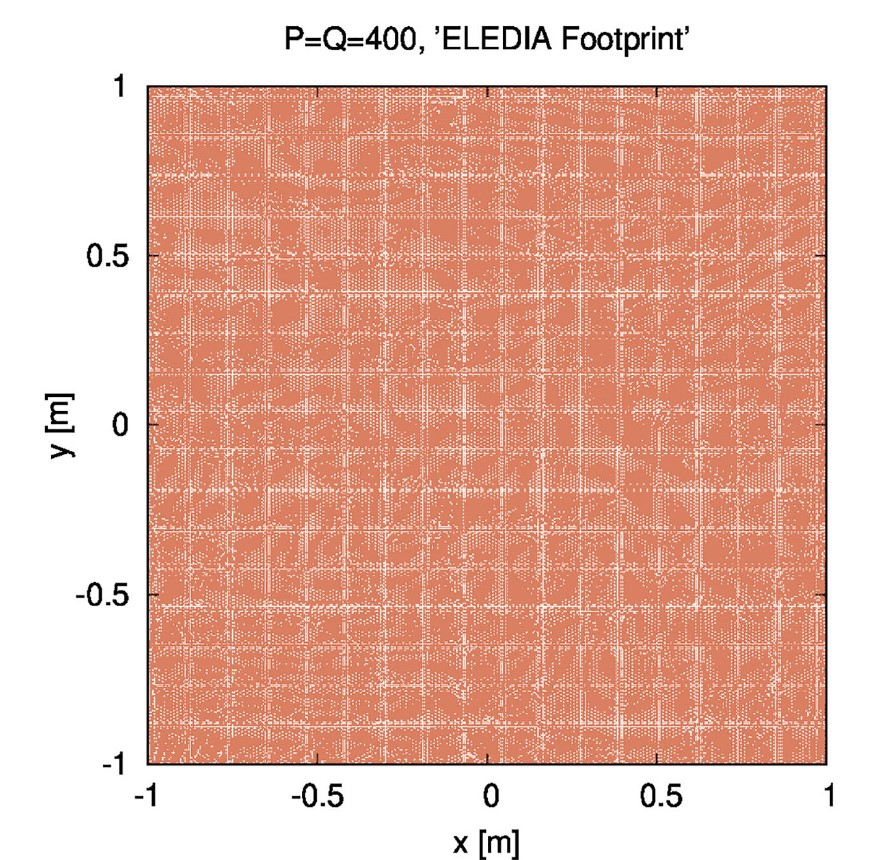
\includegraphics[scale=0.15]{./Figure/Figure25.jpg}\tabularnewline
(g)&(h)&(i)\tabularnewline
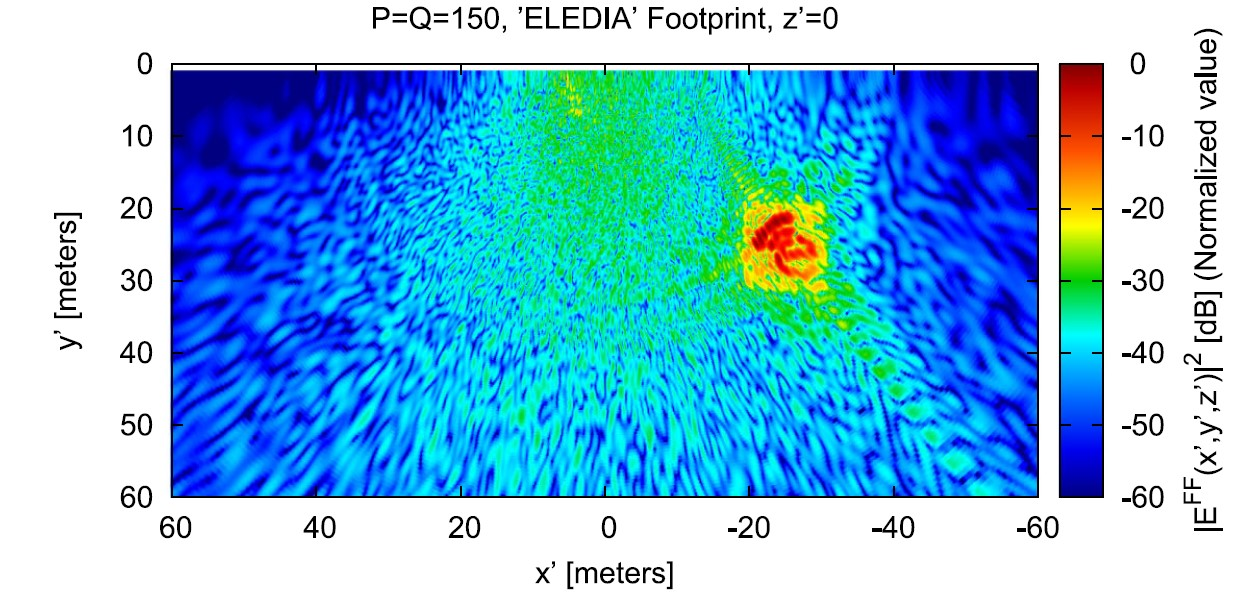
\includegraphics[scale=0.15]{./Figure/Figure29.jpg}&
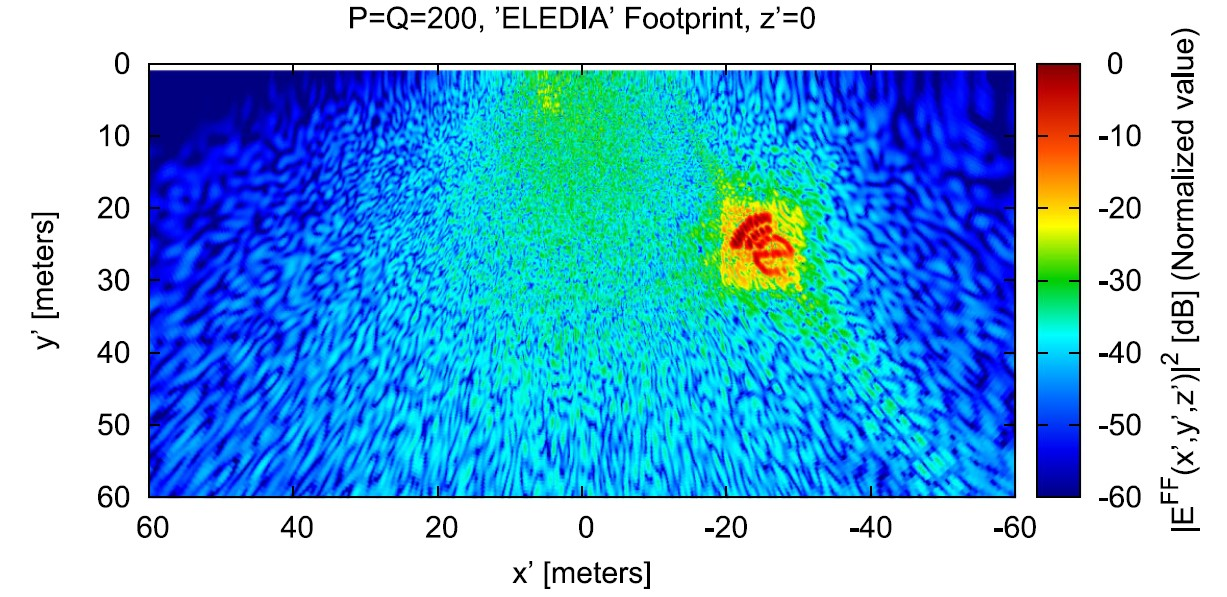
\includegraphics[scale=0.15]{./Figure/Figure30.jpg}&
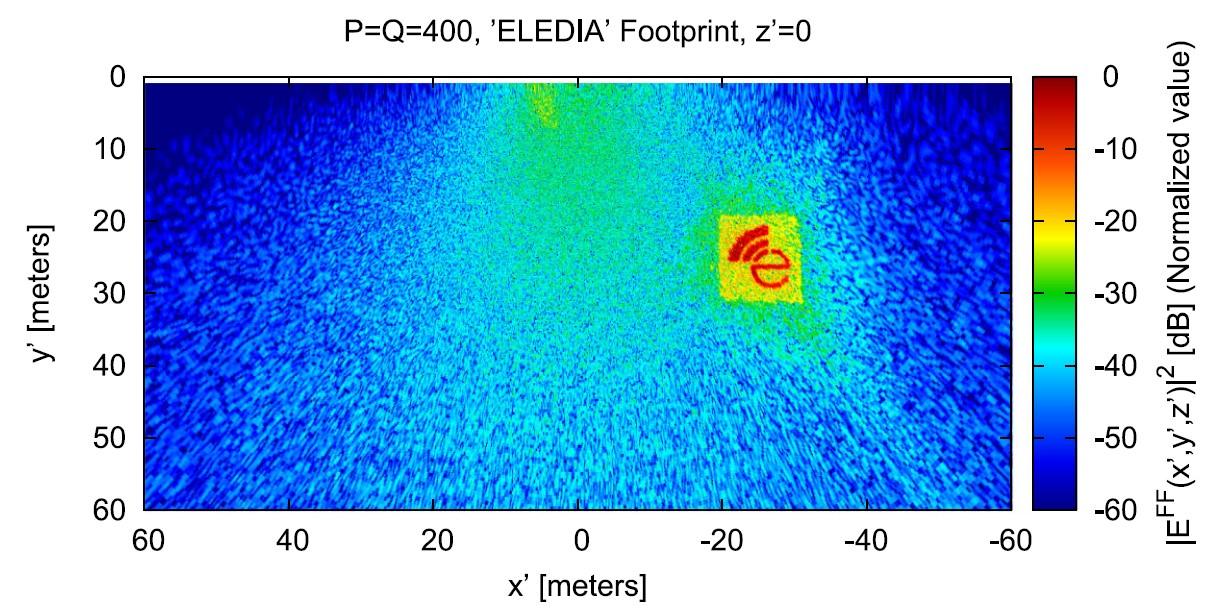
\includegraphics[scale=0.15]{./Figure/Figure31.jpg}\tabularnewline
(l)&(m)&(n)\tabularnewline
\end{longtable}\end{center}


\caption{\footnotesize\label{cap:ELEDIA_Footprint1} Numerical Validation (\emph{{}``ELEDIA''}
\emph{Footprint}) - Layout of synthesized \emph{SPSS} (First and Third
Column) and footprint patterns radiated in the observation region
$\Theta$(Second and Forth Column) by the \emph{SPSS} when $P=Q=25,50,100,150,200,400$.}
\end{figure}
As seen from Fig.\ref{cap:ELEDIA_Footprint1},
the more unit cells we have, $P$ and $Q$, the more precise the footprint
pattern is going to be. 

With the help of the figures from \ref{cap:Checkerboard_Image1}, \ref{cap:IEEE_Image1},
\ref{cap:Table1} and \ref{cap:ELEDIA_Footprint1},
we can address the cost functions:

\begin{figure}[H]
\begin{center}\begin{tabular}{cc}
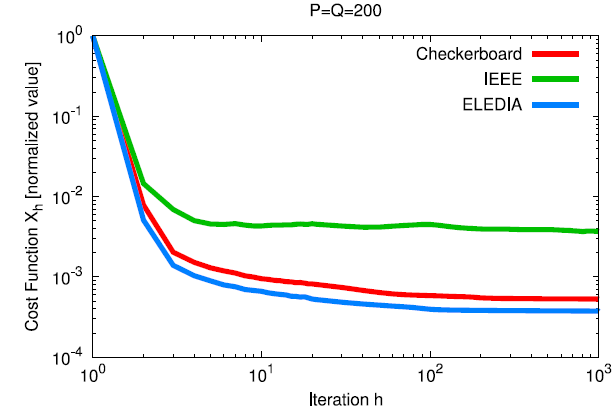
\includegraphics[%
  scale=0.3]{./Figure/Figure15.png}&
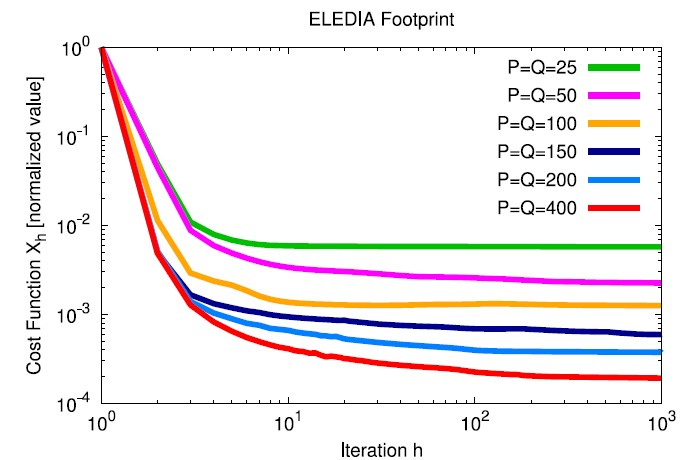
\includegraphics[%
  scale=0.3]{./Figure/Figure32.jpg}\tabularnewline
(a)&
(b)\tabularnewline
\multicolumn{2}{c}{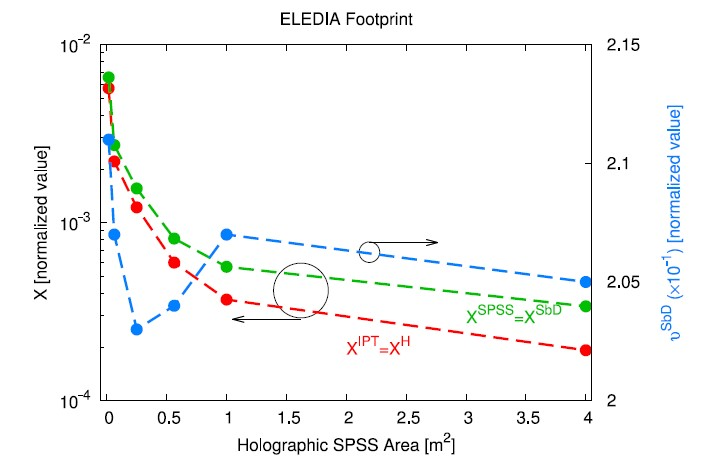
\includegraphics[%
  scale=0.3]{./Figure/Figure33.jpg}}\tabularnewline
\multicolumn{2}{c}{(c)}\tabularnewline
\end{tabular}\end{center}

\vspace{-20pt}
\caption{\footnotesize\footnotesize\label{cap:Cost_F}Numerical Validation (\emph{{}``Checkerboard''},
\emph{{}``IEEE''} and \emph{{}``ELEDIA''} footprints) - Plot of
(a) the evolution of the \emph{IPT} cost function for between the
three kinds of footprints, (b) the evolution fo the \emph{IPT} cost
function for all {}``ELEDIA'' footprints and (c) the matching indexes
{[}$\mathcal{X}^{SPSS}=\mathcal{X}^{SbD}$ (green line), $v^{SbD}$
(blue line) and $\mathcal{X}^{IPT}$ (red line){]} versus the \emph{SPSS}
size. }
\end{figure}
      \chapter{Conclusioni}
\label{cha:conclusioni}
Lorem ipsum dolor sit amet, consectetur adipiscing elit. Donec sed nunc orci. Aliquam nec nisl vitae sapien pulvinar dictum quis non urna. Suspendisse at dui a erat aliquam vestibulum. Quisque ultrices pellentesque pellentesque. Pellentesque egestas quam sed blandit tempus. Sed congue nec risus posuere euismod. Maecenas ut lacus id mauris sagittis egestas a eu dui. Class aptent taciti sociosqu ad litora torquent per conubia nostra, per inceptos himenaeos. Pellentesque at ultrices tellus. Ut eu purus eget sem iaculis ultricies sed non lorem. Curabitur gravida dui eget ex vestibulum venenatis. Phasellus gravida tellus velit, non eleifend justo lobortis eget. 


      %\input{capitolo4}
      
      
    \endgroup


    % bibliografia in formato bibtex
    %
    % aggiunta del capitolo nell'indice
    \addcontentsline{toc}{chapter}{Bibliografia}
    % stile con ordinamento alfabetico in funzione degli autori
    \bibliographystyle{plain}
    \bibliography{biblio}
%%%%%%%%%%%%%%%%%%%%%%%%%%%%%%%%%%%%%%%%%%%%%%%%%%%%%%%%%%%%%%%%%%%%%%%%%%
%%%%%%%%%%%%%%%%%%%%%%%%%%%%%%%%%%%%%%%%%%%%%%%%%%%%%%%%%%%%%%%%%%%%%%%%%%
%% Nota
%%%%%%%%%%%%%%%%%%%%%%%%%%%%%%%%%%%%%%%%%%%%%%%%%%%%%%%%%%%%%%%%%%%%%%%%%%
%% Nella bibliografia devono essere riportati tutte le fonti consultate 
%% per lo svolgimento della tesi. La bibliografia deve essere redatta 
%% in ordine alfabetico sul cognome del primo autore. 
%% 
%% La forma della citazione bibliografica va inserita secondo la fonte utilizzata:
%% 
%% LIBRI
%% Cognome e iniziale del nome autore/autori, la data di edizione, titolo, casa editrice, eventuale numero dell’edizione. 
%% 
%% ARTICOLI DI RIVISTA
%% Cognome e iniziale del nome autore/autori, titolo articolo, titolo rivista, volume, numero, numero di pagine.
%% 
%% ARTICOLI DI CONFERENZA
%% Cognome e iniziale del nome autore/autori (anno), titolo articolo, titolo conferenza, luogo della conferenza (città e paese), date della conferenza, numero di pagine. 
%% 
%% SITOGRAFIA
%% La sitografia contiene un elenco di indirizzi Web consultati e disposti in ordine alfabetico. 
%% E’ necessario:
%%   Copiare la URL (l’indirizzo web) specifica della pagina consultata
%%   Se disponibile, indicare il cognome e nome dell’autore, il titolo ed eventuale sottotitolo del testo
%%   Se disponibile, inserire la data di ultima consultazione della risorsa (gg/mm/aaaa).    
%%%%%%%%%%%%%%%%%%%%%%%%%%%%%%%%%%%%%%%%%%%%%%%%%%%%%%%%%%%%%%%%%%%%%%%%%%
%%%%%%%%%%%%%%%%%%%%%%%%%%%%%%%%%%%%%%%%%%%%%%%%%%%%%%%%%%%%%%%%%%%%%%%%%%
    

    \titleformat{\chapter}
        {\normalfont\Huge\bfseries}{Allegato \thechapter}{1em}{}
    % sezione Allegati - opzionale
    \appendix
    \chapter{Titolo primo allegato}

Lorem ipsum dolor sit amet, consectetur adipiscing elit. Donec sed nunc orci. Aliquam nec nisl vitae sapien pulvinar dictum quis non urna. Suspendisse at dui a erat aliquam vestibulum. Quisque ultrices pellentesque pellentesque. Pellentesque egestas quam sed blandit tempus. Sed congue nec risus posuere euismod. Maecenas ut lacus id mauris sagittis egestas a eu dui. Class aptent taciti sociosqu ad litora torquent per conubia nostra, per inceptos himenaeos. Pellentesque at ultrices tellus. Ut eu purus eget sem iaculis ultricies sed non lorem. Curabitur gravida dui eget ex vestibulum venenatis. Phasellus gravida tellus velit, non eleifend justo lobortis eget. 

\section{Titolo}
Lorem ipsum dolor sit amet, consectetur adipiscing elit. Donec sed nunc orci. Aliquam nec nisl vitae sapien pulvinar dictum quis non urna. Suspendisse at dui a erat aliquam vestibulum. Quisque ultrices pellentesque pellentesque. Pellentesque egestas quam sed blandit tempus. Sed congue nec risus posuere euismod. Maecenas ut lacus id mauris sagittis egestas a eu dui. Class aptent taciti sociosqu ad litora torquent per conubia nostra, per inceptos himenaeos. Pellentesque at ultrices tellus. Ut eu purus eget sem iaculis ultricies sed non lorem. Curabitur gravida dui eget ex vestibulum venenatis. Phasellus gravida tellus velit, non eleifend justo lobortis eget. 

\subsection{Sottotitolo}
Lorem ipsum dolor sit amet, consectetur adipiscing elit. Donec sed nunc orci. Aliquam nec nisl vitae sapien pulvinar dictum quis non urna. Suspendisse at dui a erat aliquam vestibulum. Quisque ultrices pellentesque pellentesque. Pellentesque egestas quam sed blandit tempus. Sed congue nec risus posuere euismod. Maecenas ut lacus id mauris sagittis egestas a eu dui. Class aptent taciti sociosqu ad litora torquent per conubia nostra, per inceptos himenaeos. Pellentesque at ultrices tellus. Ut eu purus eget sem iaculis ultricies sed non lorem. Curabitur gravida dui eget ex vestibulum venenatis. Phasellus gravida tellus velit, non eleifend justo lobortis eget. 


\chapter{Titolo secondo allegato}

Lorem ipsum dolor sit amet, consectetur adipiscing elit. Donec sed nunc orci. Aliquam nec nisl vitae sapien pulvinar dictum quis non urna. Suspendisse at dui a erat aliquam vestibulum. Quisque ultrices pellentesque pellentesque. Pellentesque egestas quam sed blandit tempus. Sed congue nec risus posuere euismod. Maecenas ut lacus id mauris sagittis egestas a eu dui. Class aptent taciti sociosqu ad litora torquent per conubia nostra, per inceptos himenaeos. Pellentesque at ultrices tellus. Ut eu purus eget sem iaculis ultricies sed non lorem. Curabitur gravida dui eget ex vestibulum venenatis. Phasellus gravida tellus velit, non eleifend justo lobortis eget. 

\section{Titolo}
Lorem ipsum dolor sit amet, consectetur adipiscing elit. Donec sed nunc orci. Aliquam nec nisl vitae sapien pulvinar dictum quis non urna. Suspendisse at dui a erat aliquam vestibulum. Quisque ultrices pellentesque pellentesque. Pellentesque egestas quam sed blandit tempus. Sed congue nec risus posuere euismod. Maecenas ut lacus id mauris sagittis egestas a eu dui. Class aptent taciti sociosqu ad litora torquent per conubia nostra, per inceptos himenaeos. Pellentesque at ultrices tellus. Ut eu purus eget sem iaculis ultricies sed non lorem. Curabitur gravida dui eget ex vestibulum venenatis. Phasellus gravida tellus velit, non eleifend justo lobortis eget. 

\subsection{Sottotitolo}
Lorem ipsum dolor sit amet, consectetur adipiscing elit. Donec sed nunc orci. Aliquam nec nisl vitae sapien pulvinar dictum quis non urna. Suspendisse at dui a erat aliquam vestibulum. Quisque ultrices pellentesque pellentesque. Pellentesque egestas quam sed blandit tempus. Sed congue nec risus posuere euismod. Maecenas ut lacus id mauris sagittis egestas a eu dui. Class aptent taciti sociosqu ad litora torquent per conubia nostra, per inceptos himenaeos. Pellentesque at ultrices tellus. Ut eu purus eget sem iaculis ultricies sed non lorem. Curabitur gravida dui eget ex vestibulum venenatis. Phasellus gravida tellus velit, non eleifend justo lobortis eget. 




\end{document}
